% Options for packages loaded elsewhere
\PassOptionsToPackage{unicode}{hyperref}
\PassOptionsToPackage{hyphens}{url}
\documentclass[
]{book}
\usepackage{xcolor}
\usepackage{amsmath,amssymb}
\setcounter{secnumdepth}{5}
\usepackage{iftex}
\ifPDFTeX
  \usepackage[T1]{fontenc}
  \usepackage[utf8]{inputenc}
  \usepackage{textcomp} % provide euro and other symbols
\else % if luatex or xetex
  \usepackage{unicode-math} % this also loads fontspec
  \defaultfontfeatures{Scale=MatchLowercase}
  \defaultfontfeatures[\rmfamily]{Ligatures=TeX,Scale=1}
\fi
\usepackage{lmodern}
\ifPDFTeX\else
  % xetex/luatex font selection
\fi
% Use upquote if available, for straight quotes in verbatim environments
\IfFileExists{upquote.sty}{\usepackage{upquote}}{}
\IfFileExists{microtype.sty}{% use microtype if available
  \usepackage[]{microtype}
  \UseMicrotypeSet[protrusion]{basicmath} % disable protrusion for tt fonts
}{}
\makeatletter
\@ifundefined{KOMAClassName}{% if non-KOMA class
  \IfFileExists{parskip.sty}{%
    \usepackage{parskip}
  }{% else
    \setlength{\parindent}{0pt}
    \setlength{\parskip}{6pt plus 2pt minus 1pt}}
}{% if KOMA class
  \KOMAoptions{parskip=half}}
\makeatother
\usepackage{color}
\usepackage{fancyvrb}
\newcommand{\VerbBar}{|}
\newcommand{\VERB}{\Verb[commandchars=\\\{\}]}
\DefineVerbatimEnvironment{Highlighting}{Verbatim}{commandchars=\\\{\}}
% Add ',fontsize=\small' for more characters per line
\usepackage{framed}
\definecolor{shadecolor}{RGB}{248,248,248}
\newenvironment{Shaded}{\begin{snugshade}}{\end{snugshade}}
\newcommand{\AlertTok}[1]{\textcolor[rgb]{0.94,0.16,0.16}{#1}}
\newcommand{\AnnotationTok}[1]{\textcolor[rgb]{0.56,0.35,0.01}{\textbf{\textit{#1}}}}
\newcommand{\AttributeTok}[1]{\textcolor[rgb]{0.13,0.29,0.53}{#1}}
\newcommand{\BaseNTok}[1]{\textcolor[rgb]{0.00,0.00,0.81}{#1}}
\newcommand{\BuiltInTok}[1]{#1}
\newcommand{\CharTok}[1]{\textcolor[rgb]{0.31,0.60,0.02}{#1}}
\newcommand{\CommentTok}[1]{\textcolor[rgb]{0.56,0.35,0.01}{\textit{#1}}}
\newcommand{\CommentVarTok}[1]{\textcolor[rgb]{0.56,0.35,0.01}{\textbf{\textit{#1}}}}
\newcommand{\ConstantTok}[1]{\textcolor[rgb]{0.56,0.35,0.01}{#1}}
\newcommand{\ControlFlowTok}[1]{\textcolor[rgb]{0.13,0.29,0.53}{\textbf{#1}}}
\newcommand{\DataTypeTok}[1]{\textcolor[rgb]{0.13,0.29,0.53}{#1}}
\newcommand{\DecValTok}[1]{\textcolor[rgb]{0.00,0.00,0.81}{#1}}
\newcommand{\DocumentationTok}[1]{\textcolor[rgb]{0.56,0.35,0.01}{\textbf{\textit{#1}}}}
\newcommand{\ErrorTok}[1]{\textcolor[rgb]{0.64,0.00,0.00}{\textbf{#1}}}
\newcommand{\ExtensionTok}[1]{#1}
\newcommand{\FloatTok}[1]{\textcolor[rgb]{0.00,0.00,0.81}{#1}}
\newcommand{\FunctionTok}[1]{\textcolor[rgb]{0.13,0.29,0.53}{\textbf{#1}}}
\newcommand{\ImportTok}[1]{#1}
\newcommand{\InformationTok}[1]{\textcolor[rgb]{0.56,0.35,0.01}{\textbf{\textit{#1}}}}
\newcommand{\KeywordTok}[1]{\textcolor[rgb]{0.13,0.29,0.53}{\textbf{#1}}}
\newcommand{\NormalTok}[1]{#1}
\newcommand{\OperatorTok}[1]{\textcolor[rgb]{0.81,0.36,0.00}{\textbf{#1}}}
\newcommand{\OtherTok}[1]{\textcolor[rgb]{0.56,0.35,0.01}{#1}}
\newcommand{\PreprocessorTok}[1]{\textcolor[rgb]{0.56,0.35,0.01}{\textit{#1}}}
\newcommand{\RegionMarkerTok}[1]{#1}
\newcommand{\SpecialCharTok}[1]{\textcolor[rgb]{0.81,0.36,0.00}{\textbf{#1}}}
\newcommand{\SpecialStringTok}[1]{\textcolor[rgb]{0.31,0.60,0.02}{#1}}
\newcommand{\StringTok}[1]{\textcolor[rgb]{0.31,0.60,0.02}{#1}}
\newcommand{\VariableTok}[1]{\textcolor[rgb]{0.00,0.00,0.00}{#1}}
\newcommand{\VerbatimStringTok}[1]{\textcolor[rgb]{0.31,0.60,0.02}{#1}}
\newcommand{\WarningTok}[1]{\textcolor[rgb]{0.56,0.35,0.01}{\textbf{\textit{#1}}}}
\usepackage{longtable,booktabs,array}
\usepackage{calc} % for calculating minipage widths
% Correct order of tables after \paragraph or \subparagraph
\usepackage{etoolbox}
\makeatletter
\patchcmd\longtable{\par}{\if@noskipsec\mbox{}\fi\par}{}{}
\makeatother
% Allow footnotes in longtable head/foot
\IfFileExists{footnotehyper.sty}{\usepackage{footnotehyper}}{\usepackage{footnote}}
\makesavenoteenv{longtable}
\usepackage{graphicx}
\makeatletter
\newsavebox\pandoc@box
\newcommand*\pandocbounded[1]{% scales image to fit in text height/width
  \sbox\pandoc@box{#1}%
  \Gscale@div\@tempa{\textheight}{\dimexpr\ht\pandoc@box+\dp\pandoc@box\relax}%
  \Gscale@div\@tempb{\linewidth}{\wd\pandoc@box}%
  \ifdim\@tempb\p@<\@tempa\p@\let\@tempa\@tempb\fi% select the smaller of both
  \ifdim\@tempa\p@<\p@\scalebox{\@tempa}{\usebox\pandoc@box}%
  \else\usebox{\pandoc@box}%
  \fi%
}
% Set default figure placement to htbp
\def\fps@figure{htbp}
\makeatother
\setlength{\emergencystretch}{3em} % prevent overfull lines
\providecommand{\tightlist}{%
  \setlength{\itemsep}{0pt}\setlength{\parskip}{0pt}}
\usepackage[]{natbib}
\bibliographystyle{plainnat}
\usepackage{bookmark}
\IfFileExists{xurl.sty}{\usepackage{xurl}}{} % add URL line breaks if available
\urlstyle{same}
\hypersetup{
  pdftitle={Machine Learning for Biostatistics},
  pdfauthor={Armando Teixeira-Pinto, Jaroslaw Harezlak \& Andrew Grant},
  hidelinks,
  pdfcreator={LaTeX via pandoc}}

\title{Machine Learning for Biostatistics}
\usepackage{etoolbox}
\makeatletter
\providecommand{\subtitle}[1]{% add subtitle to \maketitle
  \apptocmd{\@title}{\par {\large #1 \par}}{}{}
}
\makeatother
\subtitle{Module 7}
\author{Armando Teixeira-Pinto, Jaroslaw Harezlak \& Andrew Grant}
\date{2025-09-15}

\begin{document}
\maketitle

{
\setcounter{tocdepth}{1}
\tableofcontents
}
\chapter*{Unsupervised Learning}\label{unsupervised-learning}
\addcontentsline{toc}{chapter}{Unsupervised Learning}

\section*{Introduction}\label{introduction}
\addcontentsline{toc}{section}{Introduction}

\textbf{Supervised learning}, in machine learning, refers to methods that are applied
when we want to estimate the function \(f(X)\)
that relates a group of predictors \(X\) to a measured outcome \(Y\).
\textbf{Unsupervised learning } refers to methods that \emph{learn} from the data but
there is no observed outcome.

In this module, we will cover several unsupervised learning methods, namely
principal components analysis, k-means clustering and hierarchical clustering.

By the end of this module you should be able to:

\begin{enumerate}
\def\labelenumi{\arabic{enumi}.}
\tightlist
\item
  Implement dimension reduction using principal components analysis
\item
  Implement clustering methods
\end{enumerate}

\section*{Dataset used in the examples}\label{dataset-used-in-the-examples}
\addcontentsline{toc}{section}{Dataset used in the examples}

\begin{center}\rule{0.5\linewidth}{0.5pt}\end{center}

The dataset \emph{fat} is available in the \emph{library(faraway)}. You may need to install
this library.

The data set contains several physical measurements of 252 males.
Most of the variables can be measured with a scale or tape measure.
Can they be used to predict the percentage of body fat? If so,
this offers an easy alternative to an underwater weighing technique.

Data frame with 252 observations on the following 19 variables.

The data were generously supplied by Dr.~A. Garth Fisher, Human
Performance Research Center, Brigham Young University, Provo, Utah
84602, who gave permission to freely distribute the data and use them
for non-commercial purposes. Reference to the data is made in Penrose,
et al.~(1985).

Variables:

\begin{itemize}
\tightlist
\item
  brozek -- Percent body fat using Brozek's equation, 457/Density - 414.2
\item
  siri -- Percent body fat using Siri's equation, 495/Density - 450
\item
  density -- Density (gm/cm\^{}2)
\item
  age -- Age (yrs)
\item
  weight -- Weight (lbs)
\item
  height -- Height (inches)
\item
  adipos -- BMI Adiposity index = Weight/Height\^{}2 (kg/m\^{}2)
\item
  free -- Fat Free Weight = (1 - fraction of body fat) * Weight, using Brozek's formula (lbs)
\item
  neck -- Neck circumference (cm)
\item
  chest -- Chest circumference (cm)
\item
  abdom -- Abdomen circumference (cm) ``at the umbilicus and level with the iliac crest''
\item
  hip -- Hip circumference (cm)
\item
  dthigh -- Thigh circumference (cm)
\item
  knee -- Knee circumference (cm)
\item
  ankle -- Ankle circumference (cm)
\item
  biceps -- Extended biceps circumference (cm)
\item
  forearm -- Forearm circumference (cm)
\item
  wrist -- Wrist circumference (cm) ``distal to the styloid processes''
\end{itemize}

\begin{center}\rule{0.5\linewidth}{0.5pt}\end{center}

The dataset \href{https://www.dropbox.com/s/vp44yozebx5xgok/bdiag.csv?dl=0}{bdiag.csv}
contains quantitative information from digitized images of a diagnostic test
(fine needle aspirate (FNA) test on breast mass) for the diagnosis of breast
cancer. The variables describe characteristics of the cell nuclei present in
the image.

Variables Information:

\begin{itemize}
\tightlist
\item
  ID number
\item
  Diagnosis (M = malignant, B = benign)
\end{itemize}

and ten real-valued features are computed for each cell nucleus:

\begin{itemize}
\tightlist
\item
  radius (mean of distances from center to points on the perimeter)
\item
  texture (standard deviation of gray-scale values)
\item
  perimeter
\item
  area
\item
  smoothness (local variation in radius lengths)
\item
  compactness (perimeter\^{}2 / area - 1.0)
\item
  concavity (severity of concave portions of the contour)
\item
  concave points (number of concave portions of the contour)
\item
  symmetry
\item
  fractal dimension (``coastline approximation'' - 1)
\end{itemize}

The mean, standard error and ``worst'' or largest (mean of the three
largest values) of these features were computed for each image,
resulting in 30 features. For instance, field 3 is Mean Radius, field
13 is Radius SE, field 23 is Worst Radius.

This database is also available through the UW CS ftp server:
ftp ftp.cs.wisc.edu
cd math-prog/cpo-dataset/machine-learn/WDBC/

\section*{Slides from the videos}\label{slides-from-the-videos}
\addcontentsline{toc}{section}{Slides from the videos}

You can download the slides used in the videos from Unsupervised Learning:

\href{https://www.dropbox.com/scl/fi/ag3ubg9bmgn7thg58fsmb/Module-7-Unsupervised-Learning_2025.pdf?rlkey=s8ar3xlql1rmsmdvggdirnzkd&st=zgk187fy&dl=1}{Slides}

\chapter{Principal components analysis}\label{principal-components-analysis}

\section{Introduction}\label{PCA1}

Principal components analysis (PCA) is a data reduction (also referred to as
dimension reduction) technique. Given a
large set of variables, PCA identifies a small number of linear combinations
(components) that retain most of the information of the variables.

Suppose we have \(p\) variables \(x_1,...,x_p\). A PCA analysis would identify,
\(z_1,z_2,...\) components that are linear combinations of the original variables,
\[
\begin{aligned}
z_1 = \phi_{11}x_1 + &\phi_{21}x_2 +... + \phi_{p1}x_p\\
z_2 = \phi_{12}x_1 + &\phi_{22}x_2 +... + \phi_{p2}x_p\\
z_3 = \phi_{13}x_1 + &\phi_{23}x_2 +... + \phi_{p3}x_p\\
\vdots
\end{aligned}
\]

We will have up to \(p\) components (unless the number of observations is less
than \(p\)), but hopefully the first components will explain most of the
information and we can discard the others. This is why PCA is called a data
reduction method. There are two extreme situations: all the variables were
completely independent and in this case, the number of ``important'' components
would be the same as the number of variables, or all the variable are
perfectly correlated so 1 component would retain all the information.

For simplicity, let's assume that variables \(x_1,...,x_p\) are scaled to have
standard deviation 1 and mean 0. For the first component,

\[
z_1 = \phi_{11}x_1 + \phi_{21}x_2 +... + \phi_{p1}x_p\\
\]

we need to find the
\textbf{component loading vector} \((\phi_{11}, \phi_{21},... \phi_{p1})\) that
has the largest variance. We want to constrain \(\sum_{j1}^{p}{\phi^2_{j1}=1}\)
otherwise the variance would increase just by increasing the magnitude of the
\(\phi_{j1}\)'s.

Formally, we want to find the loading vector that \(\text{maximises }  var(z_1)\)
subject to \(\sum_{j1}^{p}{\phi^2_{j1}=1}\).
Given that \(z_1\) has mean zero,

\[
\begin{aligned}
\text{maximise }  var(z_1) &= \text{maximise }  \frac{1}{n}\sum_{i=1}^{n}z^2_{ij} \\
&= \text{maximise }  \frac{1}{n}\sum_{i=1}^{n} \left(\sum_{j=1}^{p}\phi_{j1}x_{ij}. \right)^2
\end{aligned}
\]

Geometrically the \(z_1\) is a projection of the vectors \(x_1,...,x_p\) into a
real line. We want this projection to have the direction that
maximises the variance. Consider the figure below representing only
2 variables \(x_1,x_2\). The first
component, is the line where the projected points have higher dispersion
(variance). The points projected on the line in the right, show a higher
variance than the one in the left.

\pandocbounded{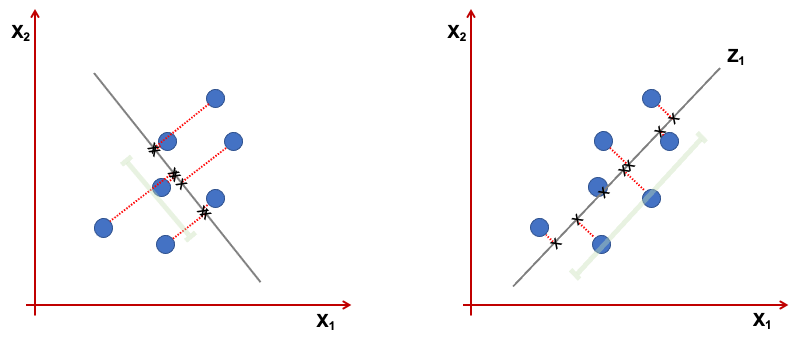
\includegraphics[keepaspectratio]{pca.png}}
\href{pca.gif}{}

Once we have found the first component, the next ones are found in a similar
fashion but with the additional requirement of orthogonality, i.e., the
components need to be independent of each other (orthogonal).

The solution for the maximisation problem above is found using eigen
decomposition where the eigenvectors are the
components of the PCA.

PCA can be used to see how variables get ``clustered'' together into the
components and how groups are characterised in terms of the components. More
commonly, PCA is used as a \textbf{pre-processing} step to reduce the dimensionality
of the data and then the main components are used in a classification or
regression algorithm.

The following is an \textbf{external video} produced by Dr.~Josh Starmer, creator
of the channel StatQuest. It gives a simple overview of the geometrical
construction of the PCA that might be useful before you do the readings.

\section{Readings}\label{PCA2}

Read the following chapters of \emph{An introduction to statistical learning}:

\begin{itemize}
\tightlist
\item
  6.3 Dimension Reduction Methods - excluding 6.3.2
\item
  12.2 Principal Components Analysis
\end{itemize}

\section{Practice session}\label{PCA3}

\subsection*{Task 1 - Identify the principal components}\label{task-1---identify-the-principal-components}
\addcontentsline{toc}{subsection}{Task 1 - Identify the principal components}

Using the \href{https://www.dropbox.com/s/vp44yozebx5xgok/bdiag.csv?dl=1}{bdiag.csv}, let's run a PCA for several characteristics of cells.
\ldots{}

\begin{Shaded}
\begin{Highlighting}[]
\CommentTok{\#libraries that we will need}
\FunctionTok{set.seed}\NormalTok{(}\DecValTok{1974}\NormalTok{) }\CommentTok{\#fix the random generator seed }
\end{Highlighting}
\end{Shaded}

\begin{Shaded}
\begin{Highlighting}[]
\CommentTok{\#read the dataset}
\NormalTok{bdiag.data }\OtherTok{\textless{}{-}} \FunctionTok{read.csv}\NormalTok{(}\StringTok{"https://www.dropbox.com/s/fvj7774lmyneab6/bdiag.csv?dl=1"}\NormalTok{, }
           \AttributeTok{stringsAsFactors =} \ConstantTok{TRUE}\NormalTok{)}

\NormalTok{bdiag.pca.data }\OtherTok{\textless{}{-}}\NormalTok{ bdiag.data[,}\FunctionTok{c}\NormalTok{(}\StringTok{"radius\_mean"}\NormalTok{, }\StringTok{"texture\_mean"}\NormalTok{, }
\StringTok{"perimeter\_mean"}\NormalTok{, }\StringTok{"area\_mean"}\NormalTok{, }\StringTok{"smoothness\_mean"}\NormalTok{, }\StringTok{"compactness\_mean"}\NormalTok{, }
\StringTok{"concavity\_mean"}\NormalTok{, }\StringTok{"concave.points\_mean"}\NormalTok{, }\StringTok{"symmetry\_mean"}\NormalTok{, }\StringTok{"fractal\_dimension\_mean"}\NormalTok{)]}

\NormalTok{bdiag.pca }\OtherTok{\textless{}{-}} \FunctionTok{prcomp}\NormalTok{(bdiag.pca.data, }\AttributeTok{scale=}\ConstantTok{TRUE}\NormalTok{) }\CommentTok{\#pca with scaled variables}
\end{Highlighting}
\end{Shaded}

The \texttt{prcomp()} function will include in its results

\begin{itemize}
\tightlist
\item
  sdev - the standard deviations of the principal components
\item
  rotation - the matrix of variable loadings for the components
\item
  x - the scaled matrix of data times the factor loadings (scores as defined
  in the \emph{An introduction to statistical learning} book, page 500)
\end{itemize}

We now can see how much variance is explained by the components. We will
use some functions of the package \texttt{factoextra} to plot some of the results.
The plot representing the variance explained by the components is called the \emph{Scree Plot}.

\begin{Shaded}
\begin{Highlighting}[]
\FunctionTok{library}\NormalTok{(factoextra)}
\end{Highlighting}
\end{Shaded}

\begin{verbatim}
## Loading required package: ggplot2
\end{verbatim}

\begin{verbatim}
## Warning: package 'ggplot2' was built under R version 4.3.3
\end{verbatim}

\begin{verbatim}
## Welcome! Want to learn more? See two factoextra-related books at https://goo.gl/ve3WBa
\end{verbatim}

\begin{Shaded}
\begin{Highlighting}[]
\FunctionTok{summary}\NormalTok{(bdiag.pca) }\CommentTok{\#variance explained}
\end{Highlighting}
\end{Shaded}

\begin{verbatim}
## Importance of components:
##                           PC1    PC2     PC3    PC4     PC5     PC6     PC7
## Standard deviation     2.3406 1.5870 0.93841 0.7064 0.61036 0.35234 0.28299
## Proportion of Variance 0.5479 0.2519 0.08806 0.0499 0.03725 0.01241 0.00801
## Cumulative Proportion  0.5479 0.7997 0.88779 0.9377 0.97495 0.98736 0.99537
##                            PC8     PC9    PC10
## Standard deviation     0.18679 0.10552 0.01680
## Proportion of Variance 0.00349 0.00111 0.00003
## Cumulative Proportion  0.99886 0.99997 1.00000
\end{verbatim}

\begin{Shaded}
\begin{Highlighting}[]
\FunctionTok{fviz\_eig}\NormalTok{(bdiag.pca) }\CommentTok{\#scree plot}
\end{Highlighting}
\end{Shaded}

\pandocbounded{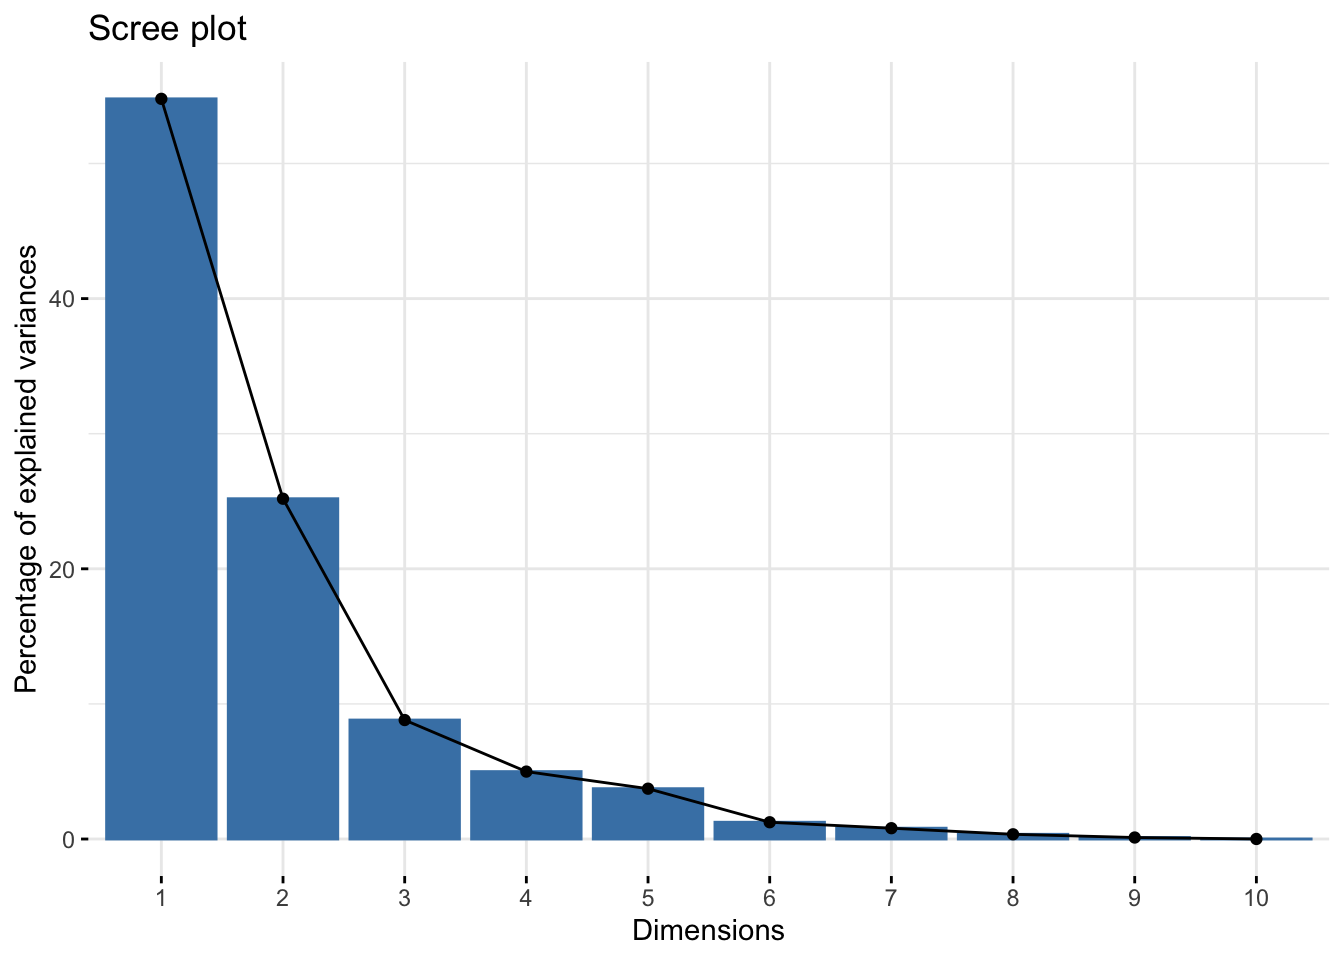
\includegraphics[keepaspectratio]{_main_files/figure-latex/unnamed-chunk-3-1.pdf}}

The first 2 components explain approximately 80\% of the total variation and
3 components, almost 90\%. The
number of components that one wants to retain is problem specific and it is
a trade-off between information and low-dimensionality.

It is also useful to look at the contribution of each variable in the different
components.

\begin{Shaded}
\begin{Highlighting}[]
 \CommentTok{\#loading vectors  }
 \FunctionTok{par}\NormalTok{(}\AttributeTok{mfrow=}\FunctionTok{c}\NormalTok{(}\DecValTok{1}\NormalTok{,}\DecValTok{3}\NormalTok{))}
 \FunctionTok{fviz\_pca\_var}\NormalTok{(bdiag.pca, }\AttributeTok{col.var =} \StringTok{"steelblue"}\NormalTok{)  }\CommentTok{\# comp 1 vs 2}
\end{Highlighting}
\end{Shaded}

\pandocbounded{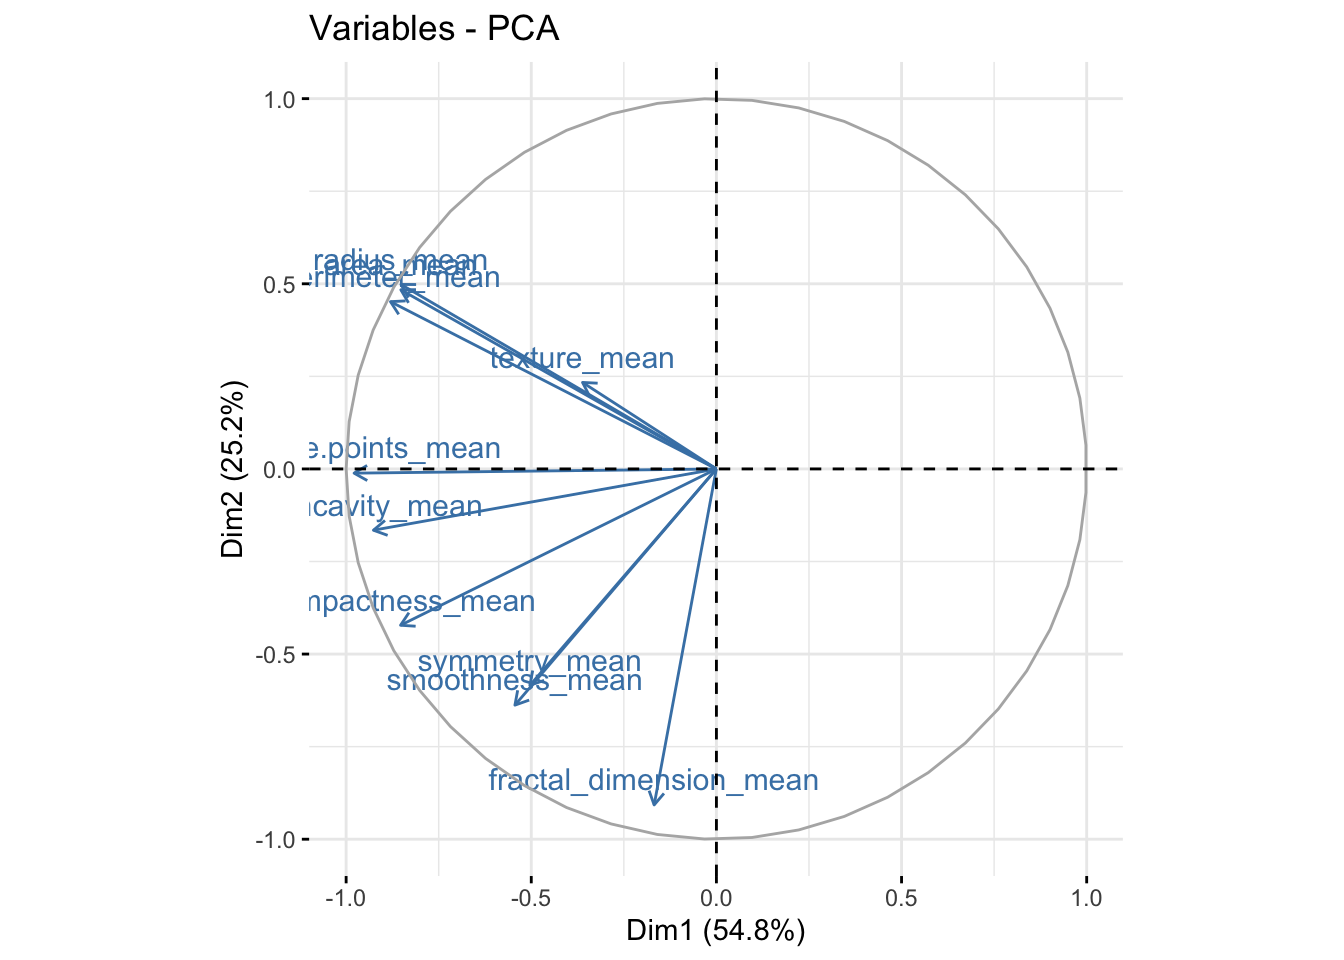
\includegraphics[keepaspectratio]{_main_files/figure-latex/unnamed-chunk-4-1.pdf}}

\begin{Shaded}
\begin{Highlighting}[]
 \FunctionTok{fviz\_pca\_var}\NormalTok{(bdiag.pca, }\AttributeTok{col.var =} \StringTok{"steelblue"}\NormalTok{,}\AttributeTok{axes=}\FunctionTok{c}\NormalTok{(}\DecValTok{1}\NormalTok{,}\DecValTok{3}\NormalTok{)) }\CommentTok{\# comp 1 vs 3}
\end{Highlighting}
\end{Shaded}

\pandocbounded{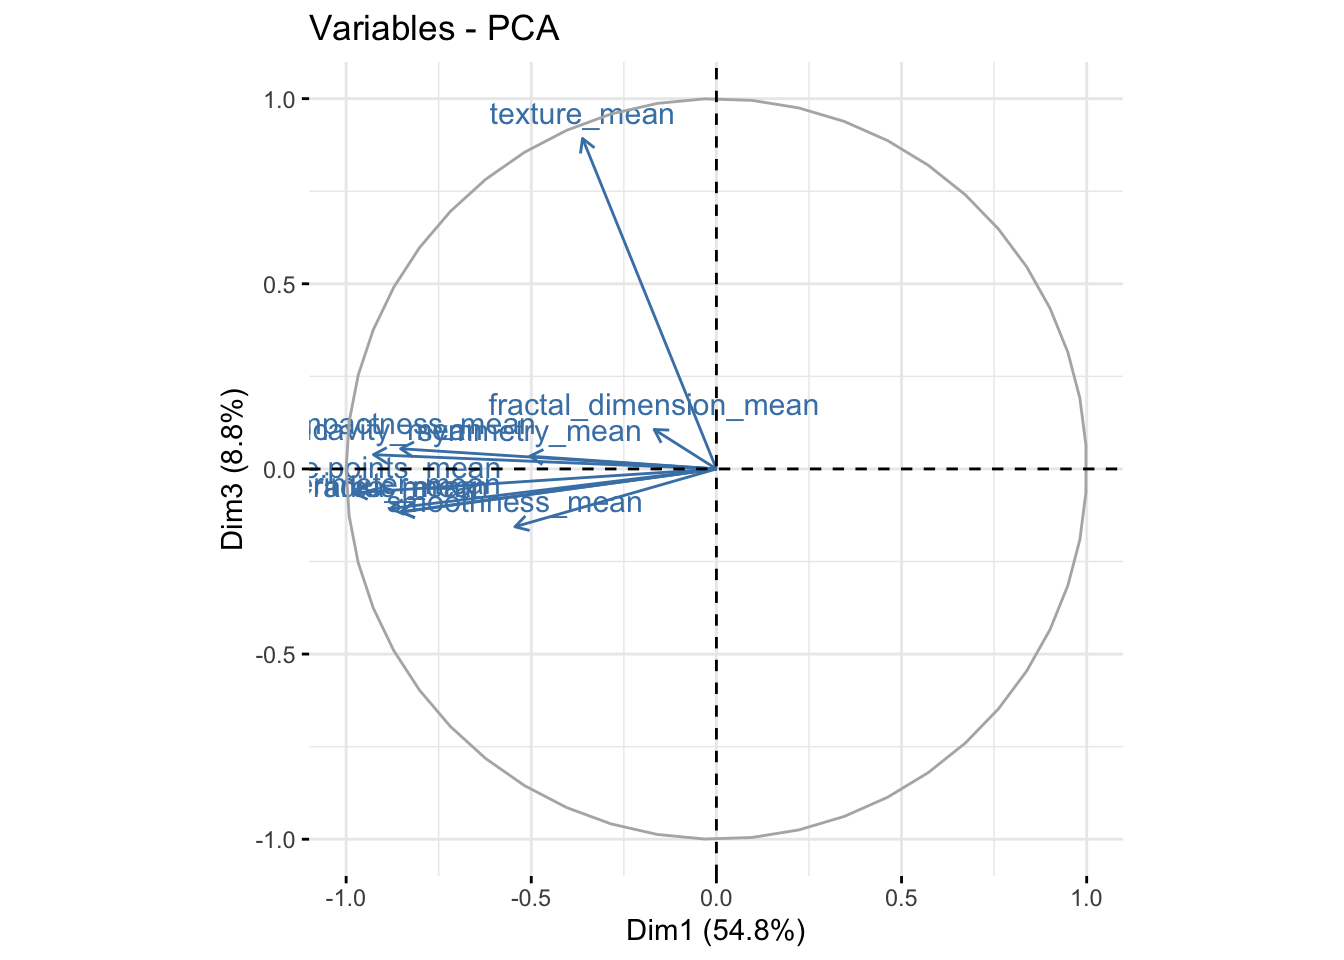
\includegraphics[keepaspectratio]{_main_files/figure-latex/unnamed-chunk-4-2.pdf}}

\begin{Shaded}
\begin{Highlighting}[]
 \FunctionTok{fviz\_pca\_var}\NormalTok{(bdiag.pca, }\AttributeTok{col.var =} \StringTok{"steelblue"}\NormalTok{,}\AttributeTok{axes=}\FunctionTok{c}\NormalTok{(}\DecValTok{2}\NormalTok{,}\DecValTok{3}\NormalTok{)) }\CommentTok{\# comp 2 vs 3}
\end{Highlighting}
\end{Shaded}

\pandocbounded{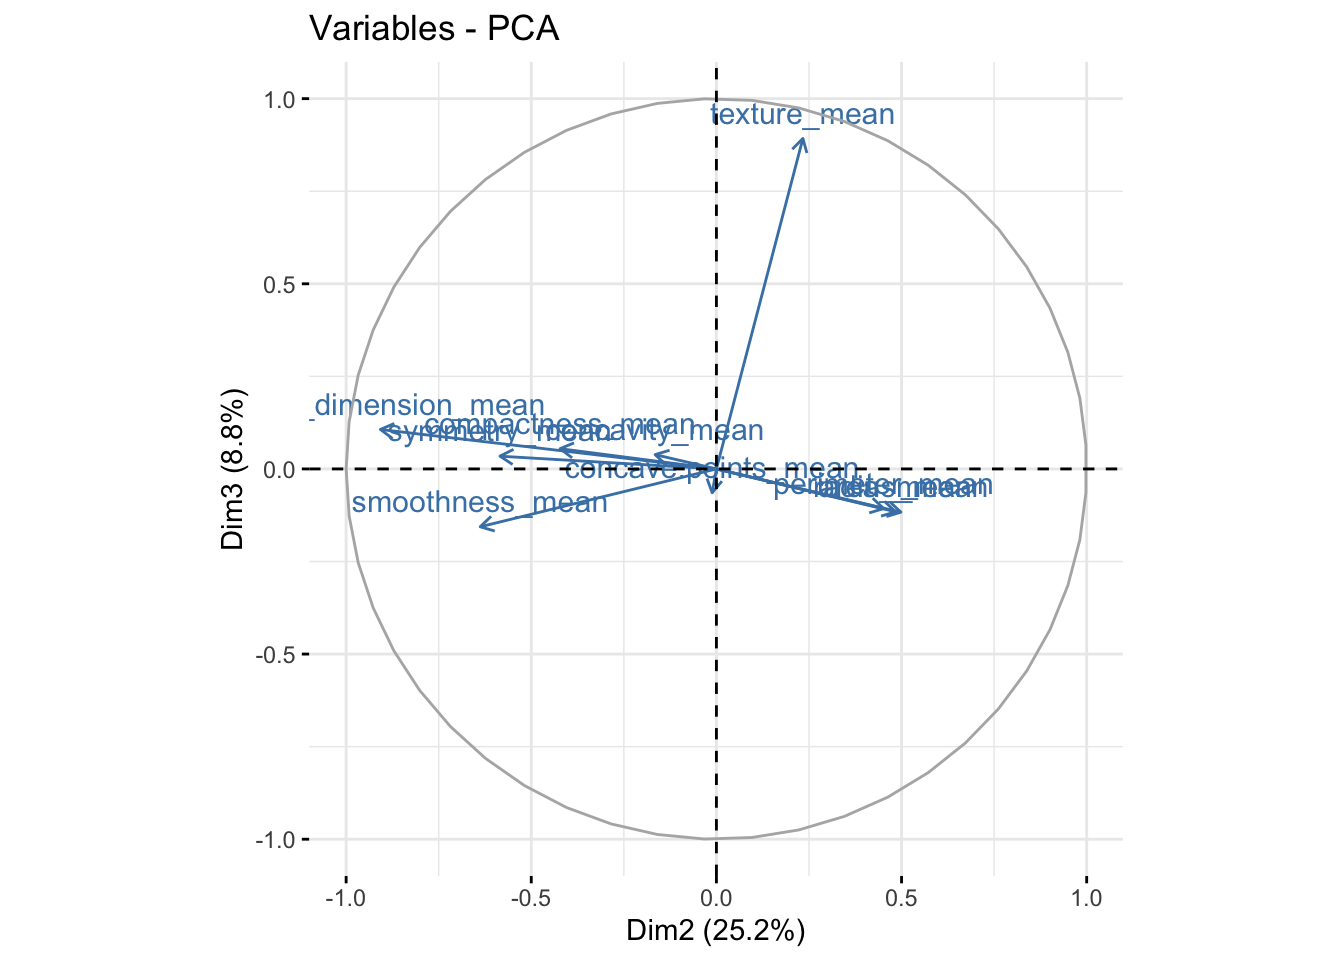
\includegraphics[keepaspectratio]{_main_files/figure-latex/unnamed-chunk-4-3.pdf}}

We can see in the plot above that among the 3 components,
\textbf{fractal\_dimension\_mean} contributes mostly
to component 2 whereas \textbf{e.points\_mean} is contributing to component 1.

\textbf{TRY IT YOURSELF:}

\begin{enumerate}
\def\labelenumi{\arabic{enumi})}
\tightlist
\item
  Get the PCA using the \texttt{eigen()} function that computes eigenvectors
  and eigenvalues for a matrix.
\end{enumerate}

See the solution code

\begin{Shaded}
\begin{Highlighting}[]
\CommentTok{\#first scale the data}
\NormalTok{bdiag.scaled }\OtherTok{\textless{}{-}} \FunctionTok{apply}\NormalTok{(bdiag.pca.data, }\DecValTok{2}\NormalTok{, scale) }\CommentTok{\#apply scale to columns}

\CommentTok{\#get the covariance matrix}
\NormalTok{cov.bdiag }\OtherTok{\textless{}{-}} \FunctionTok{cov}\NormalTok{(bdiag.scaled)}

\CommentTok{\#Get the eigenvalues and eigenvectors }
\CommentTok{\#of the covariance matrix}
\NormalTok{ev.bdiag }\OtherTok{\textless{}{-}} \FunctionTok{eigen}\NormalTok{(cov.bdiag)}

\CommentTok{\#The sqrt of the eigenvalues are the std}
\CommentTok{\#deviations of the compontents }
\FunctionTok{sqrt}\NormalTok{(ev.bdiag}\SpecialCharTok{$}\NormalTok{values)  }\CommentTok{\#equal to bdiag.pca$sdev}

\CommentTok{\#And the eigenvectors are the principal components.}
\NormalTok{ev.bdiag}\SpecialCharTok{$}\NormalTok{vector      }\CommentTok{\#equal to bdiag.pca$rotation (up to the sign)}
\end{Highlighting}
\end{Shaded}

\subsection*{Task 2 - Use PCA in a prediction model}\label{task-2---use-pca-in-a-prediction-model}
\addcontentsline{toc}{subsection}{Task 2 - Use PCA in a prediction model}

We will continue from Task 1 and use some of the principal components
as predictors in a logistic
model for the variable \textbf{diagnosis}.

The figure below shows the separations of the two diagnoses groups \emph{B} and \emph{M}
in terms of the the principal components.

\begin{Shaded}
\begin{Highlighting}[]
\NormalTok{  groups  }\OtherTok{\textless{}{-}}\NormalTok{  bdiag.data}\SpecialCharTok{$}\NormalTok{diagnosis}
  \FunctionTok{fviz\_pca\_ind}\NormalTok{(bdiag.pca,}
             \AttributeTok{col.ind =}\NormalTok{ groups, }\CommentTok{\# color by groups}
             \AttributeTok{palette =} \FunctionTok{c}\NormalTok{(}\StringTok{"\#00AFBB"}\NormalTok{,  }\StringTok{"\#FC4E07"}\NormalTok{, }\StringTok{"blue"}\NormalTok{, }\StringTok{"red"}\NormalTok{),}
             \AttributeTok{addEllipses =} \ConstantTok{TRUE}\NormalTok{, }\CommentTok{\# Concentration ellipses}
             \AttributeTok{ellipse.type =} \StringTok{"confidence"}\NormalTok{,}
             \AttributeTok{legend.title =} \StringTok{"Groups"}\NormalTok{,}
             \AttributeTok{repel =} \ConstantTok{FALSE}\NormalTok{,}
             \AttributeTok{label=}\StringTok{"none"}\NormalTok{,}
             \AttributeTok{axes=}\FunctionTok{c}\NormalTok{(}\DecValTok{1}\NormalTok{,}\DecValTok{2}\NormalTok{)}
\NormalTok{             )}
\end{Highlighting}
\end{Shaded}

\pandocbounded{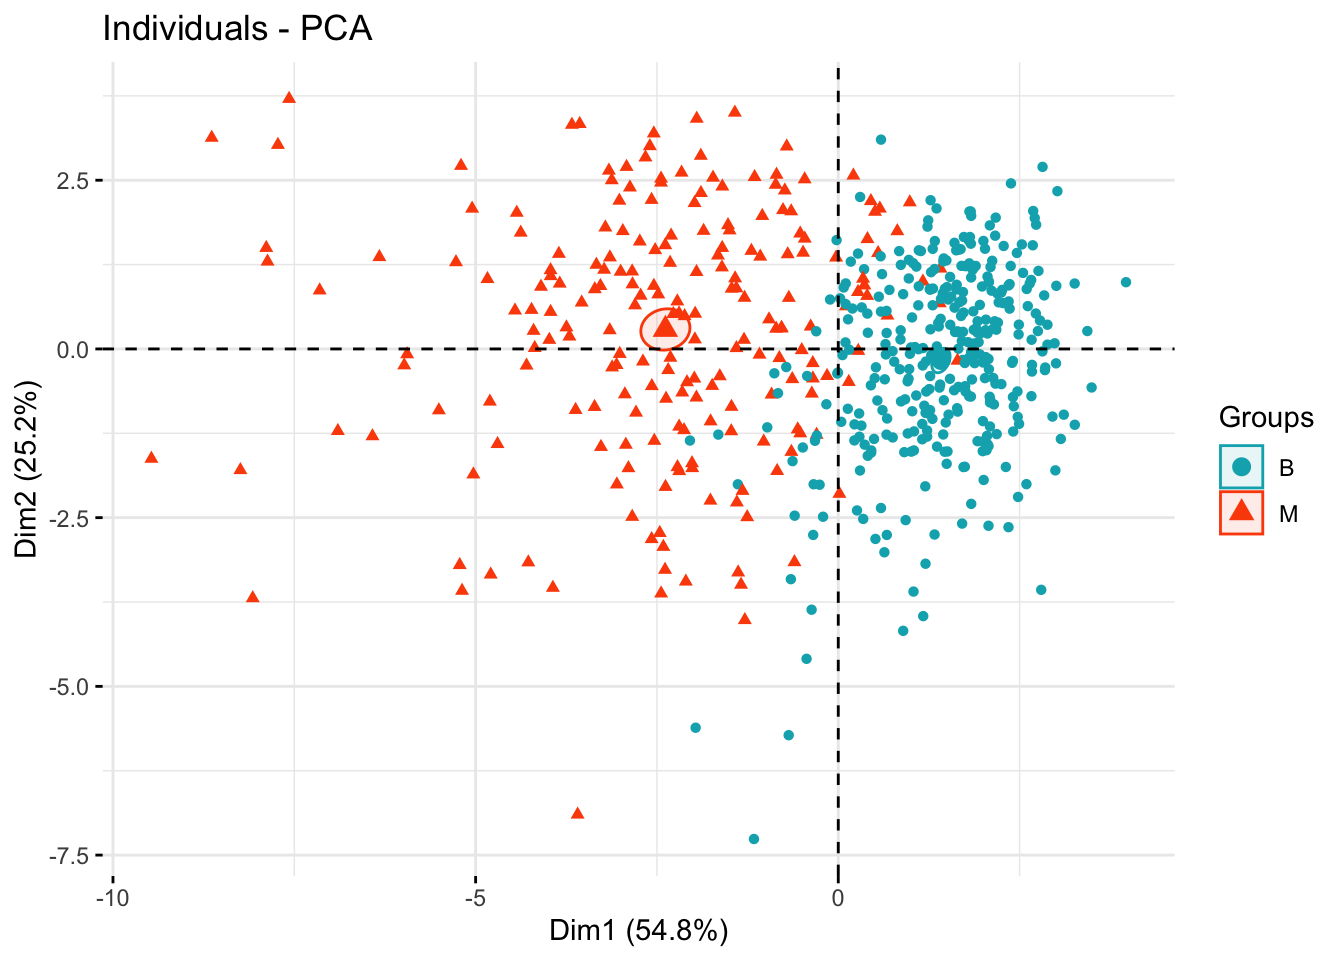
\includegraphics[keepaspectratio]{_main_files/figure-latex/unnamed-chunk-6-1.pdf}}

The package \texttt{caret} includes PCA as a pre-processing option. We will use 3
principal components to predict diagnosis

\begin{Shaded}
\begin{Highlighting}[]
\FunctionTok{library}\NormalTok{(caret)}
\end{Highlighting}
\end{Shaded}

\begin{verbatim}
## Loading required package: lattice
\end{verbatim}

\begin{verbatim}
## Registered S3 method overwritten by 'future':
##   method               from      
##   all.equal.connection parallelly
\end{verbatim}

\begin{Shaded}
\begin{Highlighting}[]
\NormalTok{trctrl }\OtherTok{\textless{}{-}} \FunctionTok{trainControl}\NormalTok{(}\AttributeTok{method =} \StringTok{"repeatedcv"}\NormalTok{, }
                       \AttributeTok{number =} \DecValTok{10}\NormalTok{,}
                       \AttributeTok{preProcOptions =}\FunctionTok{list}\NormalTok{(}\AttributeTok{pcaComp =} \DecValTok{3}\NormalTok{),  }\CommentTok{\#or list(thresh = 0.99),}
                       \AttributeTok{classProbs =} \ConstantTok{TRUE}\NormalTok{,  }
                       \AttributeTok{summaryFunction =}\NormalTok{ twoClassSummary)}

\NormalTok{bdiag.glm }\OtherTok{\textless{}{-}} \FunctionTok{train}\NormalTok{(diagnosis }\SpecialCharTok{\textasciitilde{}}\NormalTok{ radius\_mean }\SpecialCharTok{+}\NormalTok{ texture\_mean }\SpecialCharTok{+} 
\NormalTok{                     perimeter\_mean }\SpecialCharTok{+}\NormalTok{ area\_mean }\SpecialCharTok{+} 
\NormalTok{                     smoothness\_mean }\SpecialCharTok{+}\NormalTok{ compactness\_mean }\SpecialCharTok{+} 
\NormalTok{                     concavity\_mean }\SpecialCharTok{+}\NormalTok{ concave.points\_mean }\SpecialCharTok{+} 
\NormalTok{                     symmetry\_mean }\SpecialCharTok{+}\NormalTok{ fractal\_dimension\_mean,}
                   \AttributeTok{data =}\NormalTok{ bdiag.data,}
                   \AttributeTok{method =} \StringTok{"glm"}\NormalTok{,}
                   \AttributeTok{family=}\NormalTok{binomial,}
                   \AttributeTok{trControl =}\NormalTok{ trctrl,}
                   \AttributeTok{preProcess=}\FunctionTok{c}\NormalTok{(}\StringTok{"center"}\NormalTok{, }\StringTok{"scale"}\NormalTok{, }\StringTok{"pca"}\NormalTok{), }\CommentTok{\#uses PCA}
                   \AttributeTok{metric=}\StringTok{"ROC"}\NormalTok{)}

\NormalTok{bdiag.glm}
\end{Highlighting}
\end{Shaded}

\begin{verbatim}
## Generalized Linear Model 
## 
## 569 samples
##  10 predictor
##   2 classes: 'B', 'M' 
## 
## Pre-processing: centered (10), scaled (10), principal component
##  signal extraction (10) 
## Resampling: Cross-Validated (10 fold, repeated 1 times) 
## Summary of sample sizes: 512, 512, 512, 512, 512, 513, ... 
## Resampling results:
## 
##   ROC        Sens       Spec     
##   0.9834474  0.9605556  0.8863636
\end{verbatim}

The prediction accuracy is excellent with three components. We can get the
coefficients for these components but they don't have an obvious interpretation.

\begin{Shaded}
\begin{Highlighting}[]
\FunctionTok{summary}\NormalTok{(bdiag.glm)}
\end{Highlighting}
\end{Shaded}

\begin{verbatim}
## 
## Call:
## NULL
## 
## Coefficients:
##             Estimate Std. Error z value Pr(>|z|)    
## (Intercept)  -0.5911     0.2022  -2.923  0.00347 ** 
## PC1          -2.7029     0.2882  -9.379  < 2e-16 ***
## PC2           0.8271     0.1509   5.481 4.22e-08 ***
## PC3           0.7430     0.2144   3.465  0.00053 ***
## ---
## Signif. codes:  0 '***' 0.001 '**' 0.01 '*' 0.05 '.' 0.1 ' ' 1
## 
## (Dispersion parameter for binomial family taken to be 1)
## 
##     Null deviance: 751.44  on 568  degrees of freedom
## Residual deviance: 172.10  on 565  degrees of freedom
## AIC: 180.1
## 
## Number of Fisher Scoring iterations: 8
\end{verbatim}

And the principal components matrix:

\begin{Shaded}
\begin{Highlighting}[]
\NormalTok{bdiag.glm}\SpecialCharTok{$}\NormalTok{preProcess}\SpecialCharTok{$}\NormalTok{rotation}
\end{Highlighting}
\end{Shaded}

\begin{verbatim}
##                                PC1          PC2         PC3
## radius_mean            -0.36393793  0.313929073 -0.12442759
## texture_mean           -0.15445113  0.147180909  0.95105659
## perimeter_mean         -0.37604434  0.284657885 -0.11408360
## area_mean              -0.36408585  0.304841714 -0.12337786
## smoothness_mean        -0.23248053 -0.401962324 -0.16653247
## compactness_mean       -0.36444206 -0.266013147  0.05827786
## concavity_mean         -0.39574849 -0.104285968  0.04114649
## concave.points_mean    -0.41803840 -0.007183605 -0.06855383
## symmetry_mean          -0.21523797 -0.368300910  0.03672364
## fractal_dimension_mean -0.07183744 -0.571767700  0.11358395
\end{verbatim}

\textbf{TRY IT YOURSELF:}

\begin{enumerate}
\def\labelenumi{\arabic{enumi})}
\tightlist
\item
  Fit a random forest to predict \textbf{diagnosis} using 7 principal components and
  cross-validating the number of variables used in each split.
\end{enumerate}

See the solution code

\begin{Shaded}
\begin{Highlighting}[]
\NormalTok{trctrl }\OtherTok{\textless{}{-}} \FunctionTok{trainControl}\NormalTok{(}\AttributeTok{method =} \StringTok{"repeatedcv"}\NormalTok{, }
                       \AttributeTok{number =} \DecValTok{10}\NormalTok{,}
                       \AttributeTok{preProcOptions =}\FunctionTok{list}\NormalTok{(}\AttributeTok{pcaComp =} \DecValTok{7}\NormalTok{), }
                       \AttributeTok{classProbs =} \ConstantTok{TRUE}\NormalTok{,  }
                       \AttributeTok{summaryFunction =}\NormalTok{ twoClassSummary)}

\NormalTok{bdiag.rf }\OtherTok{\textless{}{-}} \FunctionTok{train}\NormalTok{(diagnosis }\SpecialCharTok{\textasciitilde{}}\NormalTok{ radius\_mean }\SpecialCharTok{+}\NormalTok{ texture\_mean }\SpecialCharTok{+} 
\NormalTok{                     perimeter\_mean }\SpecialCharTok{+}\NormalTok{ area\_mean }\SpecialCharTok{+} 
\NormalTok{                     smoothness\_mean }\SpecialCharTok{+}\NormalTok{ compactness\_mean }\SpecialCharTok{+} 
\NormalTok{                     concavity\_mean }\SpecialCharTok{+}\NormalTok{ concave.points\_mean }\SpecialCharTok{+} 
\NormalTok{                     symmetry\_mean }\SpecialCharTok{+}\NormalTok{ fractal\_dimension\_mean,}
                   \AttributeTok{data =}\NormalTok{ bdiag.data,}
                   \AttributeTok{method =} \StringTok{"rf"}\NormalTok{,}
                   \AttributeTok{family=}\NormalTok{binomial,}
                   \AttributeTok{trControl =}\NormalTok{ trctrl,}
                   \AttributeTok{preProcess=}\FunctionTok{c}\NormalTok{(}\StringTok{"center"}\NormalTok{, }\StringTok{"scale"}\NormalTok{, }\StringTok{"pca"}\NormalTok{), }\CommentTok{\#uses PCA}
                   \AttributeTok{ntree =} \DecValTok{100}\NormalTok{,}
                   \AttributeTok{tuneGrid =} \FunctionTok{expand.grid}\NormalTok{(}\AttributeTok{mtry =} \FunctionTok{c}\NormalTok{(}\DecValTok{1}\SpecialCharTok{:}\DecValTok{7}\NormalTok{)),  }
                   \AttributeTok{metric=}\StringTok{"ROC"}\NormalTok{)}

\NormalTok{bdiag.rf}
\end{Highlighting}
\end{Shaded}

\subsection*{Task 3 - Use PCA to compress an image}\label{task-3---use-pca-to-compress-an-image}
\addcontentsline{toc}{subsection}{Task 3 - Use PCA to compress an image}

This is not a typical Biostats problem, but it illustrates the idea behind PCA.
Let's consider an original image \href{https://www.dropbox.com/s/hruqk3h69p5l458/roo.jpg?dl=1}{roo.jpg}.
For simplicity we will only use the
green channel information (the original image has 3 channels: red, green
and blue). This will correspond to a black and white image.

\begin{Shaded}
\begin{Highlighting}[]
\FunctionTok{library}\NormalTok{(jpeg)}
\FunctionTok{library}\NormalTok{(graphics)}
\CommentTok{\#the jpeg has 3 channels: red,green, blue}
\CommentTok{\#for simplicity of the example, I am only}
\CommentTok{\#reading the green channlel}
\NormalTok{roo }\OtherTok{\textless{}{-}} \FunctionTok{readJPEG}\NormalTok{(}\StringTok{"roo.jpg"}\NormalTok{)[,,}\DecValTok{2}\NormalTok{]}

\CommentTok{\#You can have a look at the image}
\FunctionTok{plot}\NormalTok{(}\DecValTok{1}\SpecialCharTok{:}\DecValTok{2}\NormalTok{, }\AttributeTok{type=}\StringTok{\textquotesingle{}n\textquotesingle{}}\NormalTok{, }\AttributeTok{axes=}\NormalTok{F, }\AttributeTok{ann=}\NormalTok{F)}
\FunctionTok{rasterImage}\NormalTok{(roo, }\DecValTok{1}\NormalTok{, }\DecValTok{2}\NormalTok{, }\DecValTok{2}\NormalTok{, }\DecValTok{1}\NormalTok{)}
\end{Highlighting}
\end{Shaded}

\pandocbounded{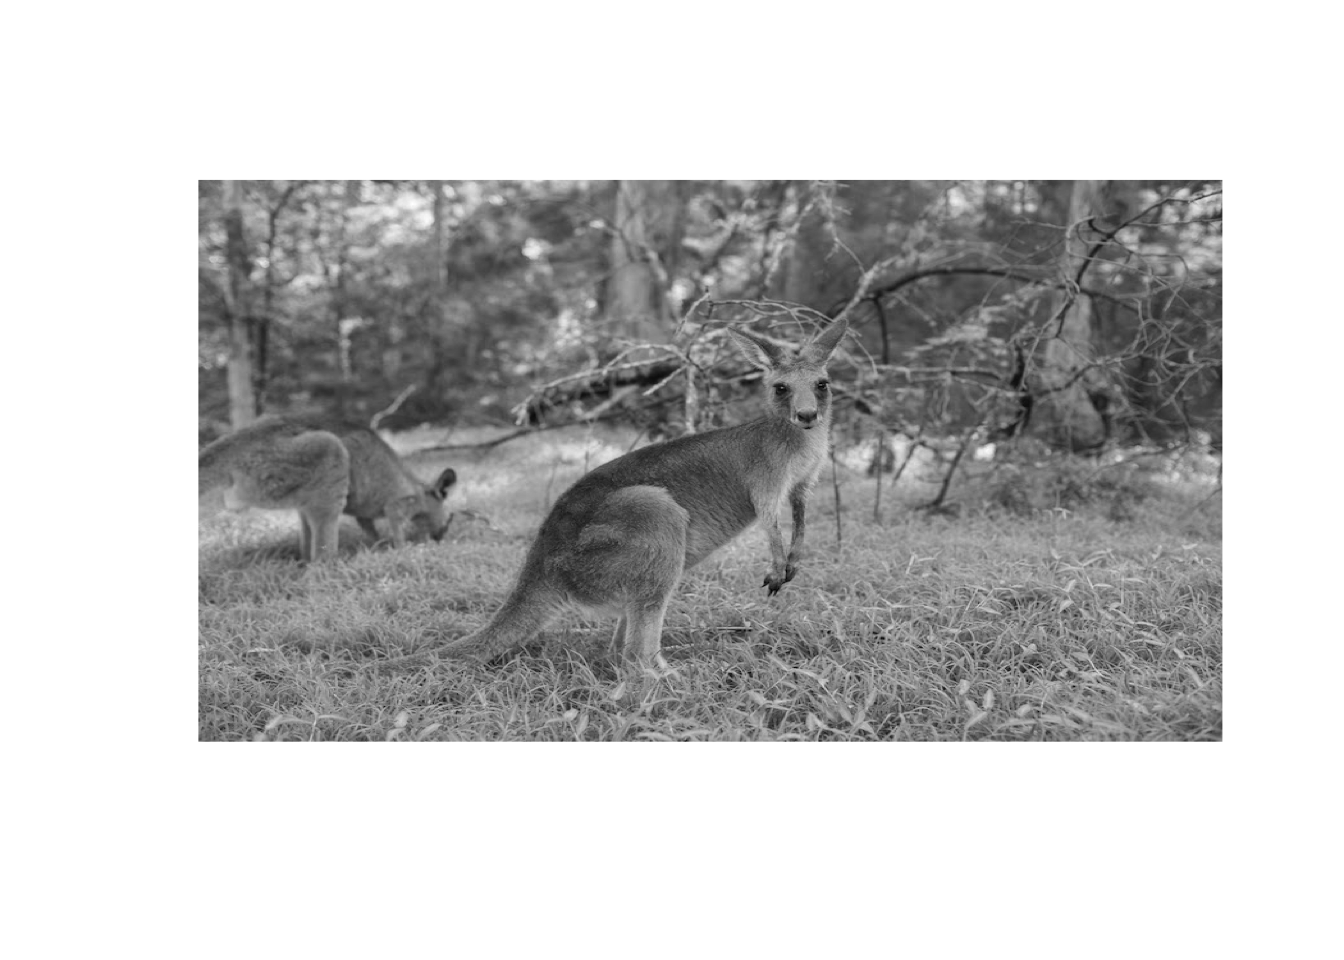
\includegraphics[keepaspectratio]{_main_files/figure-latex/roo-original-1.pdf}}

An image is a matrix of pixels with values that represent the intensity of the
the pixel, where 0=white and 1=black. In this case, the image is 800x534 pixels
as you can see by the dimension of the matrix.

\begin{Shaded}
\begin{Highlighting}[]
\FunctionTok{dim}\NormalTok{(roo)}
\end{Highlighting}
\end{Shaded}

\begin{verbatim}
## [1] 534 800
\end{verbatim}

As we would expect, there are several places in the photo where columns of
pixels are strongly correlated with adjacent columns:

\begin{Shaded}
\begin{Highlighting}[]
\FunctionTok{library}\NormalTok{(gplots)}
\end{Highlighting}
\end{Shaded}

\begin{verbatim}
## 
## Attaching package: 'gplots'
\end{verbatim}

\begin{verbatim}
## The following object is masked from 'package:stats':
## 
##     lowess
\end{verbatim}

\begin{Shaded}
\begin{Highlighting}[]
\CommentTok{\#color for the heatmap}
\NormalTok{col.correlation }\OtherTok{\textless{}{-}} \FunctionTok{colorRampPalette}\NormalTok{(}\FunctionTok{c}\NormalTok{(}\StringTok{"red"}\NormalTok{,}\StringTok{"yellow"}\NormalTok{,}\StringTok{"darkgreen"}\NormalTok{), }
                                    \AttributeTok{space =} \StringTok{"rgb"}\NormalTok{)(}\DecValTok{30}\NormalTok{)}
\FunctionTok{heatmap.2}\NormalTok{(}\FunctionTok{cor}\NormalTok{(roo), }
          \AttributeTok{Rowv =}\NormalTok{ F, }\AttributeTok{Colv =}\NormalTok{ F, }
          \AttributeTok{dendrogram =} \StringTok{"none"}\NormalTok{,}
          \AttributeTok{trace=}\StringTok{"none"}\NormalTok{, }
          \AttributeTok{col=}\NormalTok{col.correlation)}
\end{Highlighting}
\end{Shaded}

\pandocbounded{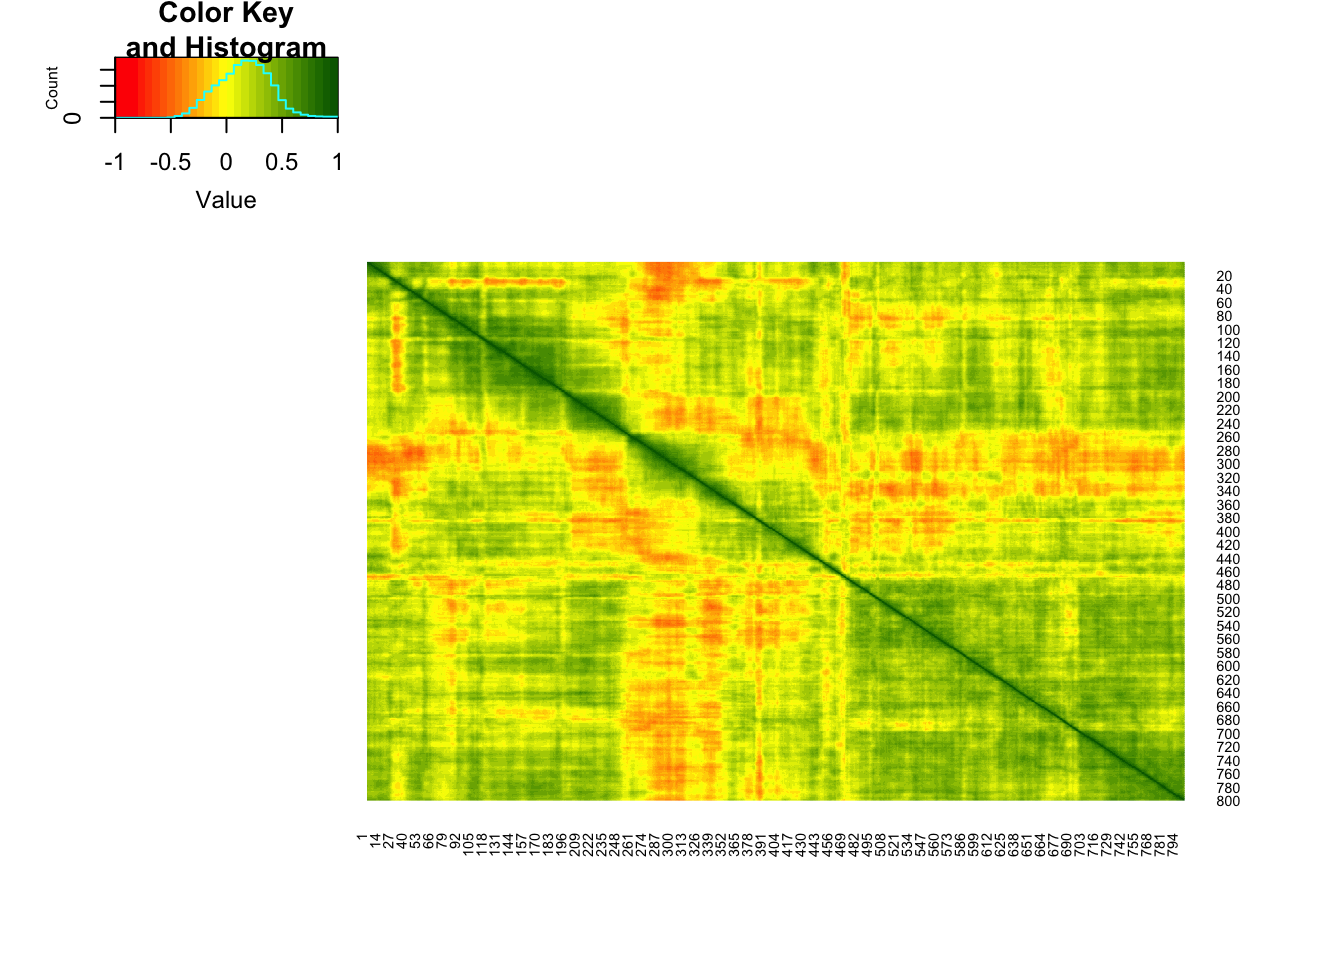
\includegraphics[keepaspectratio]{_main_files/figure-latex/unnamed-chunk-12-1.pdf}}

Therefore, PCA we should be able to reduce the original dimension (800x534)
while keeping a substantial part of the information.

Out of the 534 components, the first
10 components produce the following image.

Note: despite having 800 ``variables'' columns,
there are only 534 rows and we cannot have more components than rows. In fact,
we should only have 533 components, but given that we did not centre the data,
we have 534.

\begin{Shaded}
\begin{Highlighting}[]
\CommentTok{\#All the columns with the intensities are in the same scale so }
\CommentTok{\#we do not need to scale them}
\CommentTok{\#Also, we do not want to centre the columns otherwise}
\CommentTok{\#the values can no longer be interpreted as intensities and }
\CommentTok{\#we will not be able to plot the results}

\CommentTok{\#PCA}
\NormalTok{roo.pca }\OtherTok{\textless{}{-}} \FunctionTok{prcomp}\NormalTok{(roo, }\AttributeTok{center =} \ConstantTok{FALSE}\NormalTok{) }

\CommentTok{\#The intensities given by the first 10 components}
\NormalTok{roo.pca10 }\OtherTok{\textless{}{-}}\NormalTok{ roo.pca}\SpecialCharTok{$}\NormalTok{x[,}\DecValTok{1}\SpecialCharTok{:}\DecValTok{10}\NormalTok{] }\SpecialCharTok{\%*\%} \FunctionTok{t}\NormalTok{(roo.pca}\SpecialCharTok{$}\NormalTok{rotation[,}\DecValTok{1}\SpecialCharTok{:}\DecValTok{10}\NormalTok{])}

\CommentTok{\#this is just to make sure all the values}
\CommentTok{\#remain within 0 and 1 (due to rounding in the}
\CommentTok{\#calculation, sometimes the values go slightly higher than 1)}
\NormalTok{roo.pca10[roo.pca10}\SpecialCharTok{\textgreater{}}\DecValTok{1}\NormalTok{] }\OtherTok{\textless{}{-}}\DecValTok{1}
\NormalTok{roo.pca10[roo.pca10}\SpecialCharTok{\textless{}}\DecValTok{0}\NormalTok{] }\OtherTok{\textless{}{-}}\DecValTok{0}

\CommentTok{\#You can have a look at the image}
\FunctionTok{par}\NormalTok{(}\AttributeTok{mfrow=}\FunctionTok{c}\NormalTok{(}\DecValTok{1}\NormalTok{,}\DecValTok{2}\NormalTok{))}
\FunctionTok{plot}\NormalTok{(}\DecValTok{1}\SpecialCharTok{:}\DecValTok{2}\NormalTok{, }\AttributeTok{type=}\StringTok{\textquotesingle{}n\textquotesingle{}}\NormalTok{, }\AttributeTok{axes=}\NormalTok{F, }\AttributeTok{ann=}\NormalTok{F)}
\FunctionTok{title}\NormalTok{ (}\StringTok{"original"}\NormalTok{)}
\FunctionTok{rasterImage}\NormalTok{(roo, }\DecValTok{1}\NormalTok{, }\DecValTok{2}\NormalTok{, }\DecValTok{2}\NormalTok{, }\DecValTok{1}\NormalTok{)}

\FunctionTok{plot}\NormalTok{(}\DecValTok{1}\SpecialCharTok{:}\DecValTok{2}\NormalTok{, }\AttributeTok{type=}\StringTok{\textquotesingle{}n\textquotesingle{}}\NormalTok{, }\AttributeTok{axes=}\NormalTok{F, }\AttributeTok{ann=}\NormalTok{F)}
\FunctionTok{title}\NormalTok{(}\StringTok{"Image with 10 components from PCA"}\NormalTok{)}
\FunctionTok{rasterImage}\NormalTok{(roo.pca10, }\DecValTok{1}\NormalTok{, }\DecValTok{2}\NormalTok{, }\DecValTok{2}\NormalTok{, }\DecValTok{1}\NormalTok{)}
\end{Highlighting}
\end{Shaded}

\pandocbounded{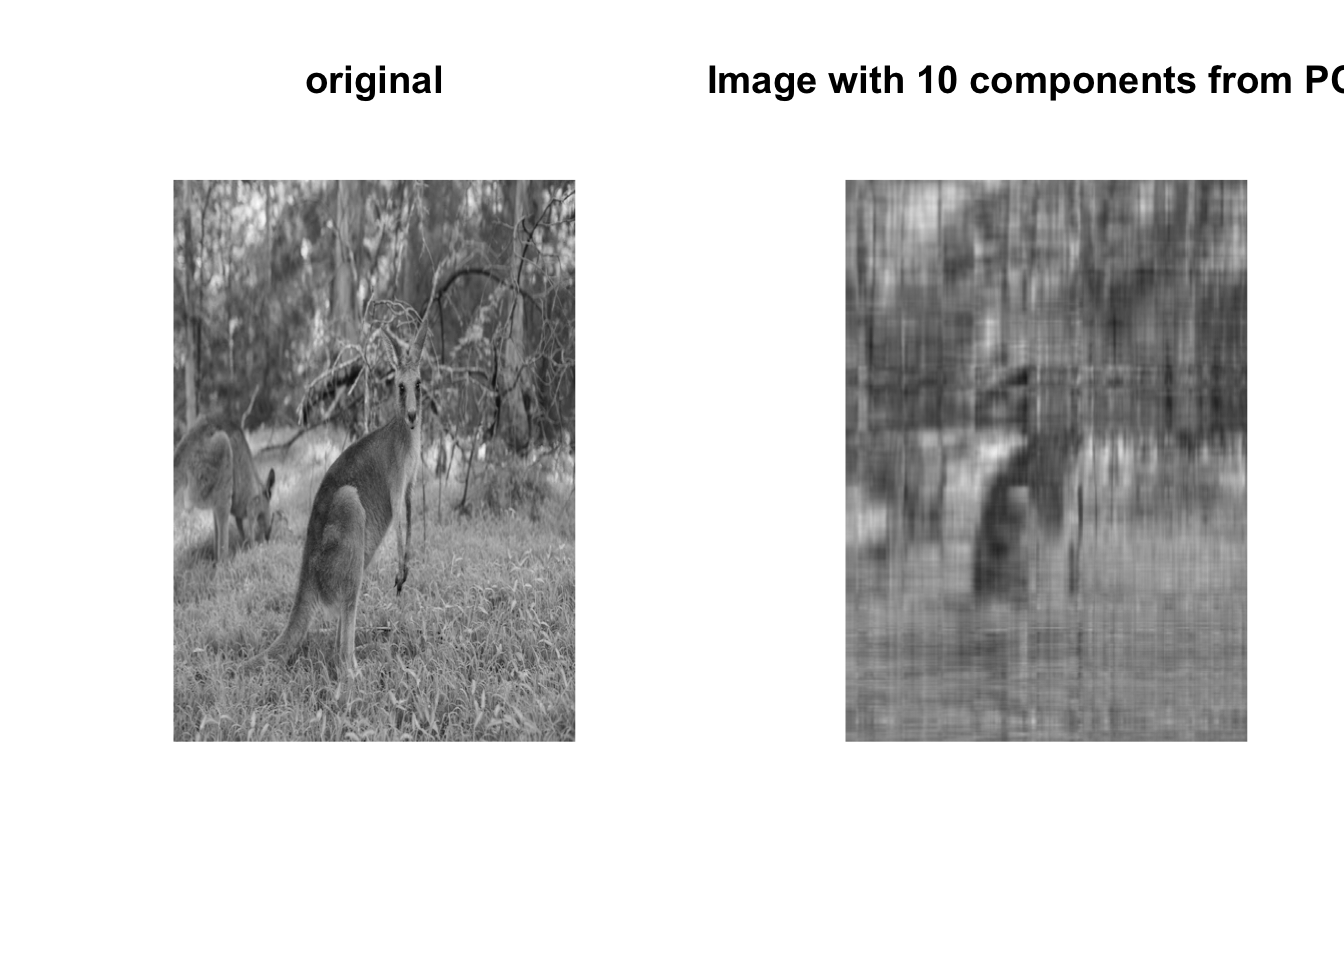
\includegraphics[keepaspectratio]{_main_files/figure-latex/unnamed-chunk-13-1.pdf}}

Notice that we are using only 10 of the 534 components. If we had used all the
components we would have the original image. Let's see the image with different
number of components

\begin{Shaded}
\begin{Highlighting}[]
\CommentTok{\# Intensities with 20, 50, 100 and 534 components}
\NormalTok{roo.pca.j }\OtherTok{\textless{}{-}} \FunctionTok{lapply}\NormalTok{(}\FunctionTok{c}\NormalTok{(}\DecValTok{20}\NormalTok{, }\DecValTok{50}\NormalTok{, }\DecValTok{100}\NormalTok{, }\DecValTok{534}\NormalTok{), }\ControlFlowTok{function}\NormalTok{(j) \{}
\NormalTok{                      jcomp }\OtherTok{\textless{}{-}}\NormalTok{ roo.pca}\SpecialCharTok{$}\NormalTok{x[,}\DecValTok{1}\SpecialCharTok{:}\NormalTok{j] }\SpecialCharTok{\%*\%} \FunctionTok{t}\NormalTok{(roo.pca}\SpecialCharTok{$}\NormalTok{rotation[,}\DecValTok{1}\SpecialCharTok{:}\NormalTok{j])}
\NormalTok{                      jcomp[jcomp}\SpecialCharTok{\textgreater{}}\DecValTok{1}\NormalTok{] }\OtherTok{\textless{}{-}}\DecValTok{1}
\NormalTok{                      jcomp[jcomp}\SpecialCharTok{\textless{}}\DecValTok{0}\NormalTok{] }\OtherTok{\textless{}{-}}\DecValTok{0}
                      \FunctionTok{return}\NormalTok{(jcomp)}
\NormalTok{                      \}}
\NormalTok{                    )}

\FunctionTok{par}\NormalTok{(}\AttributeTok{mfrow=}\FunctionTok{c}\NormalTok{(}\DecValTok{2}\NormalTok{,}\DecValTok{2}\NormalTok{))}
\FunctionTok{plot}\NormalTok{(}\DecValTok{1}\SpecialCharTok{:}\DecValTok{2}\NormalTok{, }\AttributeTok{type=}\StringTok{\textquotesingle{}n\textquotesingle{}}\NormalTok{, }\AttributeTok{axes=}\NormalTok{F, }\AttributeTok{ann=}\NormalTok{F)}
\FunctionTok{title}\NormalTok{ (}\StringTok{"20 components"}\NormalTok{)}
\FunctionTok{rasterImage}\NormalTok{(roo.pca.j[[}\DecValTok{1}\NormalTok{]], }\DecValTok{1}\NormalTok{, }\DecValTok{2}\NormalTok{, }\DecValTok{2}\NormalTok{, }\DecValTok{1}\NormalTok{)}

\FunctionTok{plot}\NormalTok{(}\DecValTok{1}\SpecialCharTok{:}\DecValTok{2}\NormalTok{, }\AttributeTok{type=}\StringTok{\textquotesingle{}n\textquotesingle{}}\NormalTok{, }\AttributeTok{axes=}\NormalTok{F, }\AttributeTok{ann=}\NormalTok{F)}
\FunctionTok{title}\NormalTok{(}\StringTok{"50 components"}\NormalTok{)}
\FunctionTok{rasterImage}\NormalTok{(roo.pca.j[[}\DecValTok{2}\NormalTok{]], }\DecValTok{1}\NormalTok{, }\DecValTok{2}\NormalTok{, }\DecValTok{2}\NormalTok{, }\DecValTok{1}\NormalTok{)}

\FunctionTok{plot}\NormalTok{(}\DecValTok{1}\SpecialCharTok{:}\DecValTok{2}\NormalTok{, }\AttributeTok{type=}\StringTok{\textquotesingle{}n\textquotesingle{}}\NormalTok{, }\AttributeTok{axes=}\NormalTok{F, }\AttributeTok{ann=}\NormalTok{F)}
\FunctionTok{title}\NormalTok{(}\StringTok{"100 components"}\NormalTok{)}
\FunctionTok{rasterImage}\NormalTok{(roo.pca.j[[}\DecValTok{3}\NormalTok{]], }\DecValTok{1}\NormalTok{, }\DecValTok{2}\NormalTok{, }\DecValTok{2}\NormalTok{, }\DecValTok{1}\NormalTok{)}

\FunctionTok{plot}\NormalTok{(}\DecValTok{1}\SpecialCharTok{:}\DecValTok{2}\NormalTok{, }\AttributeTok{type=}\StringTok{\textquotesingle{}n\textquotesingle{}}\NormalTok{, }\AttributeTok{axes=}\NormalTok{F, }\AttributeTok{ann=}\NormalTok{F)}
\FunctionTok{title}\NormalTok{(}\StringTok{"534 components (original image"}\NormalTok{)}
\FunctionTok{rasterImage}\NormalTok{(roo.pca.j[[}\DecValTok{4}\NormalTok{]], }\DecValTok{1}\NormalTok{, }\DecValTok{2}\NormalTok{, }\DecValTok{2}\NormalTok{, }\DecValTok{1}\NormalTok{)}
\end{Highlighting}
\end{Shaded}

\pandocbounded{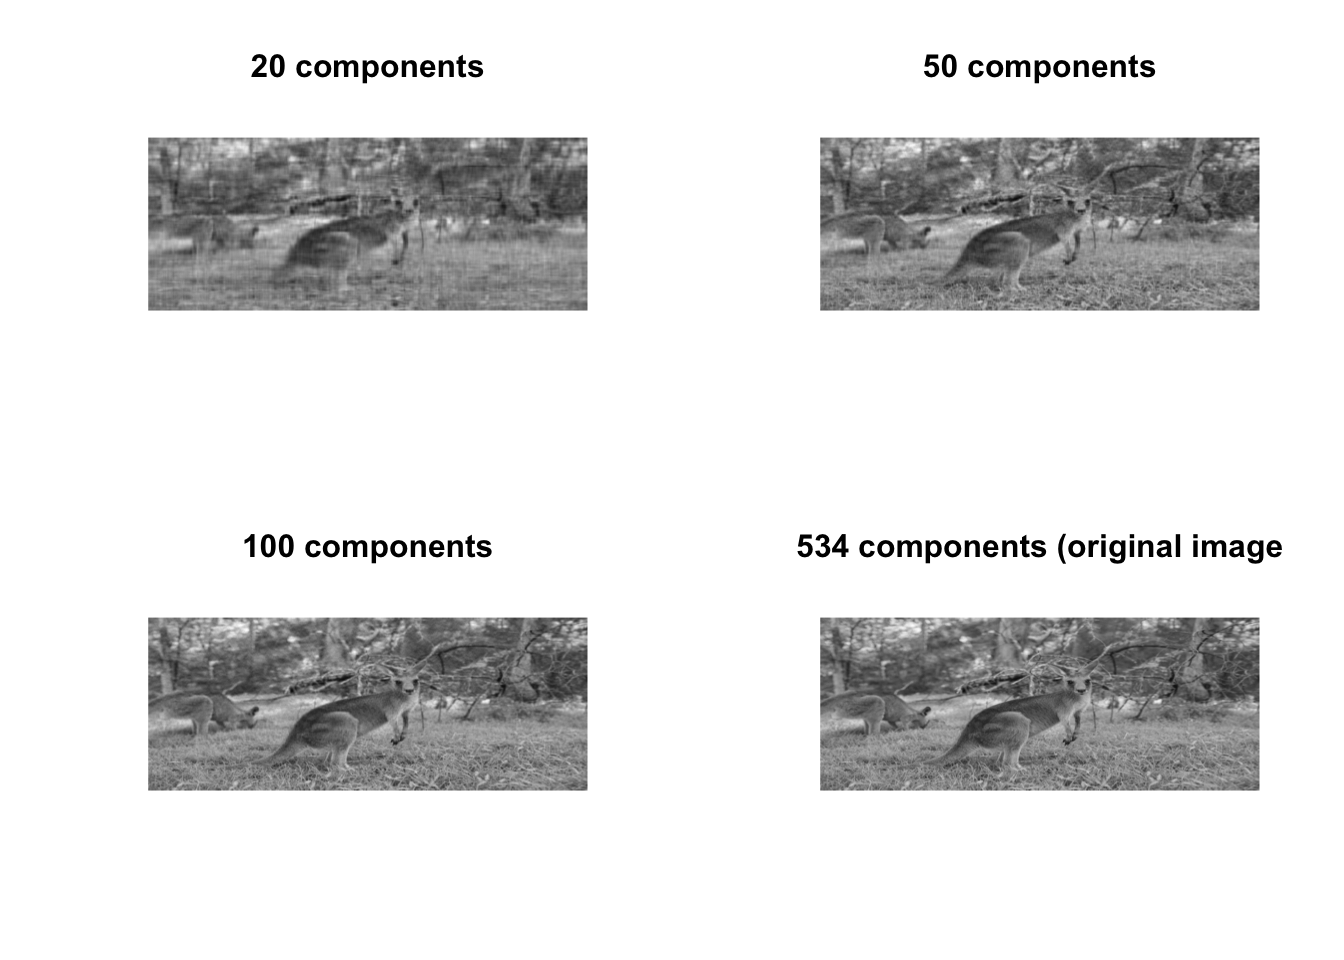
\includegraphics[keepaspectratio]{_main_files/figure-latex/unnamed-chunk-14-1.pdf}}

\textbf{TRY IT YOURSELF:}

\begin{enumerate}
\def\labelenumi{\arabic{enumi})}
\tightlist
\item
  Produce the image above with 100 components but using the colored photo.
\end{enumerate}

See the solution code

\begin{Shaded}
\begin{Highlighting}[]
\NormalTok{roo }\OtherTok{\textless{}{-}} \FunctionTok{readJPEG}\NormalTok{(}\StringTok{"roo.jpg"}\NormalTok{)}

\CommentTok{\# roo is now a list with three elements }
\CommentTok{\#corresponding to the channels RBG}
\CommentTok{\#we will do PCA in each element}
\NormalTok{roo.rbg.pca}\OtherTok{\textless{}{-}} \FunctionTok{apply}\NormalTok{(roo, }\DecValTok{3}\NormalTok{, prcomp, }\AttributeTok{center =} \ConstantTok{FALSE}\NormalTok{) }

\CommentTok{\#Computes the intensities using 100 components}
\NormalTok{roo.pca2 }\OtherTok{\textless{}{-}} \FunctionTok{lapply}\NormalTok{(roo.rbg.pca, }\ControlFlowTok{function}\NormalTok{(channel.pca) \{}
\NormalTok{                      jcomp }\OtherTok{\textless{}{-}}\NormalTok{ channel.pca}\SpecialCharTok{$}\NormalTok{x[,}\DecValTok{1}\SpecialCharTok{:}\DecValTok{100}\NormalTok{] }\SpecialCharTok{\%*\%} \FunctionTok{t}\NormalTok{(channel.pca}\SpecialCharTok{$}\NormalTok{rotation[,}\DecValTok{1}\SpecialCharTok{:}\DecValTok{100}\NormalTok{])}
\NormalTok{                      jcomp[jcomp}\SpecialCharTok{\textgreater{}}\DecValTok{1}\NormalTok{] }\OtherTok{\textless{}{-}}\DecValTok{1}
\NormalTok{                      jcomp[jcomp}\SpecialCharTok{\textless{}}\DecValTok{0}\NormalTok{] }\OtherTok{\textless{}{-}}\DecValTok{0}
                      \FunctionTok{return}\NormalTok{(jcomp)\})}

\CommentTok{\#Transforms the above list into an array}
\NormalTok{roo.pca2}\OtherTok{\textless{}{-}}\FunctionTok{array}\NormalTok{(}\FunctionTok{as.numeric}\NormalTok{(}\FunctionTok{unlist}\NormalTok{(roo.pca2)), }
               \AttributeTok{dim=}\FunctionTok{c}\NormalTok{(}\DecValTok{534}\NormalTok{, }\DecValTok{800}\NormalTok{, }\DecValTok{3}\NormalTok{))}


\CommentTok{\#You can have a look at the image}
\FunctionTok{par}\NormalTok{(}\AttributeTok{mfrow=}\FunctionTok{c}\NormalTok{(}\DecValTok{1}\NormalTok{,}\DecValTok{2}\NormalTok{))}
\FunctionTok{plot}\NormalTok{(}\DecValTok{1}\SpecialCharTok{:}\DecValTok{2}\NormalTok{, }\AttributeTok{type=}\StringTok{\textquotesingle{}n\textquotesingle{}}\NormalTok{, }\AttributeTok{axes=}\NormalTok{F, }\AttributeTok{ann=}\NormalTok{F)}
\FunctionTok{title}\NormalTok{ (}\StringTok{"original"}\NormalTok{)}
\FunctionTok{rasterImage}\NormalTok{(roo, }\DecValTok{1}\NormalTok{, }\DecValTok{2}\NormalTok{, }\DecValTok{2}\NormalTok{, }\DecValTok{1}\NormalTok{)}
\FunctionTok{plot}\NormalTok{(}\DecValTok{1}\SpecialCharTok{:}\DecValTok{2}\NormalTok{, }\AttributeTok{type=}\StringTok{\textquotesingle{}n\textquotesingle{}}\NormalTok{, }\AttributeTok{axes=}\NormalTok{F, }\AttributeTok{ann=}\NormalTok{F)}
\FunctionTok{title}\NormalTok{ (}\StringTok{"100 components"}\NormalTok{)}
\FunctionTok{rasterImage}\NormalTok{(roo.pca2, }\DecValTok{1}\NormalTok{, }\DecValTok{2}\NormalTok{, }\DecValTok{2}\NormalTok{, }\DecValTok{1}\NormalTok{)}
\end{Highlighting}
\end{Shaded}

\pandocbounded{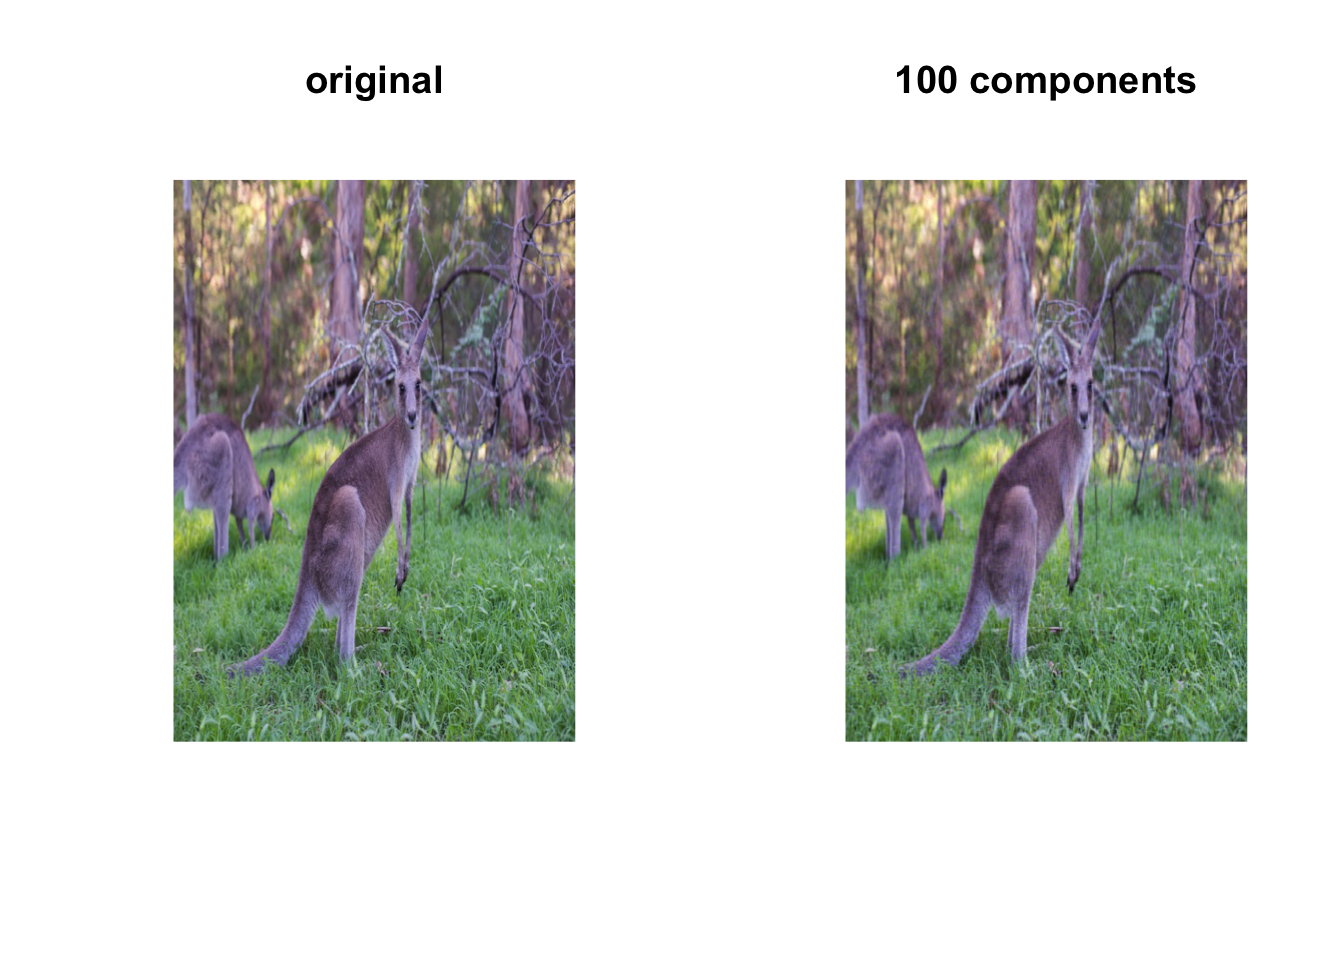
\includegraphics[keepaspectratio]{_main_files/figure-latex/unnamed-chunk-15-1.pdf}}

\section{Exercises}\label{PCA4}

Solve the following exercises:

\begin{enumerate}
\def\labelenumi{\arabic{enumi})}
\tightlist
\item
  The dataset \emph{fat} is available in the \emph{library(faraway)}.
  The dataset contains several physical measurements.
\end{enumerate}

Using the variables \emph{age}, \emph{weight}, \emph{height}, \emph{adipos}, \emph{free}, \emph{neck}, \emph{chest},
\emph{abdom}, \emph{hip}, \emph{thigh}, \emph{knee}, \emph{ankle}, \emph{biceps}, \emph{forearm} and \emph{wrist}

\begin{enumerate}
\def\labelenumi{\alph{enumi})}
\item
  How many components explain at least 95\% of the variance?
\item
  Identify 2 variable that seem to have a stronger contribution to the 2nd
  principal component.
\item
  Compare the adjusted-\(r^2\) for a linear model for \textbf{brozek} using all
  the predictors and a linear model only using 2 principal components to predict
  \textbf{brozek}.
\end{enumerate}

\chapter{K-means clustering}\label{k-means-clustering}

\section{Introduction}\label{KM1}

K-means clustering is a popular unsupervised learning method based on a
simple and intuitive approach that clusters similar observations into groups.

We start by choosing the number of clusters \(K\) and the objective is to assign
every observation to one, and just one, of the clusters. The clusters are
chosen so that the within-cluster variation is minimised, i.e., the data points
in each cluster should be close together.

The figure below shows an example of 3 clusters based on two variables.

\pandocbounded{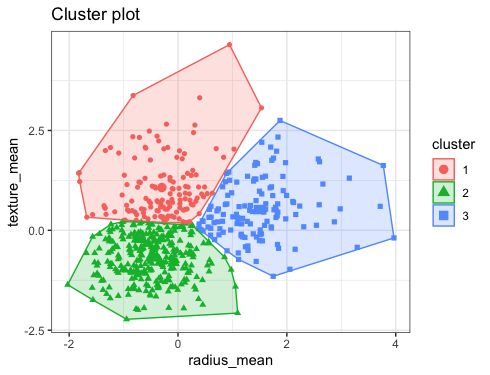
\includegraphics[keepaspectratio]{kmeans.png}}

The way the clusters are defined is based on an iterative process. Once we
chose the number of clusters:

\begin{itemize}
\tightlist
\item
  We start by assigning each data point to one of the clusters, randomly.
\item
  We then compute the centroid of each cluster.
\item
  Next, we compute the distance (usually the Euclidean distance) of each data point to the centroids.
\item
  The data points are re-assigned to the corresponding cluster
  of the closest centroid.
\item
  The centroids are recomputed
\item
  We repeat the process until convergence
\end{itemize}

One important question that immediately arises is \emph{how many clusters should
we consider?} Unfortunately, there is not a definitive answer. In the practice
session we will show some graphical methods that can be used as an indication of
the number of clusters suggested by the data, but as you will see, different
methods can suggest different number of clusters.

\section{Readings}\label{KM2}

Read the following chapters of \emph{An introduction to statistical learning}:

\begin{itemize}
\tightlist
\item
  12.4.1 K-Means Clustering Analysis
\end{itemize}

\section{Practice session}\label{KM3}

\subsection*{Task 1 - Identify k clusters}\label{task-1---identify-k-clusters}
\addcontentsline{toc}{subsection}{Task 1 - Identify k clusters}

Using the \href{https://www.dropbox.com/s/vp44yozebx5xgok/bdiag.csv?dl=1}{bdiag.csv},
let's use 2 of the variables that characterise the cell nuclei - \emph{radius\_mean}
and \emph{texture\_mean} - to identify 3 data clusters

We will use the function \texttt{kmeans()} with the option \texttt{centers=3} indicating
that we want 3 clusters.

\begin{Shaded}
\begin{Highlighting}[]
\CommentTok{\#read the dataset}
\NormalTok{bdiag.data }\OtherTok{\textless{}{-}} \FunctionTok{read.csv}\NormalTok{(}\StringTok{"https://www.dropbox.com/s/vp44yozebx5xgok/bdiag.csv?dl=1"}\NormalTok{, }
           \AttributeTok{stringsAsFactors =} \ConstantTok{TRUE}\NormalTok{)}

\CommentTok{\#select a subset of the variables}
\NormalTok{bdiag}\FloatTok{.2}\NormalTok{vars }\OtherTok{\textless{}{-}}\NormalTok{ bdiag.data[,}\FunctionTok{c}\NormalTok{(}\StringTok{"radius\_mean"}\NormalTok{, }\StringTok{"texture\_mean"}\NormalTok{)]}

\CommentTok{\#let\textquotesingle{}s compute the 3 clusters}
\NormalTok{km }\OtherTok{\textless{}{-}} \FunctionTok{kmeans}\NormalTok{(bdiag}\FloatTok{.2}\NormalTok{vars, }\AttributeTok{centers =} \DecValTok{3}\NormalTok{)}

\NormalTok{km}
\end{Highlighting}
\end{Shaded}

\begin{verbatim}
## K-means clustering with 3 clusters of sizes 123, 291, 155
## 
## Cluster means:
##   radius_mean texture_mean
## 1    19.55667     21.85732
## 2    12.43088     16.11027
## 3    13.00369     23.22110
## 
## Clustering vector:
##   [1] 2 1 1 3 1 2 1 3 3 3 3 2 1 3 3 3 3 1 1 2 2 2 2 1 1 2 3 1 3 2 1 2 1 1 2 1 3
##  [38] 2 3 3 3 3 1 3 3 1 2 2 2 3 3 2 2 1 3 2 1 3 2 2 2 3 3 2 3 3 3 2 2 2 1 2 1 2
##  [75] 2 1 2 2 1 2 3 2 1 1 2 1 3 1 3 2 3 3 2 2 3 1 2 3 2 3 3 2 3 2 2 2 2 2 1 3 2
## [112] 3 3 3 2 3 2 2 3 1 2 1 1 2 2 2 3 1 2 1 2 3 1 2 1 3 2 2 2 2 2 2 2 2 2 2 2 2
## [149] 2 2 3 3 2 2 2 2 1 1 2 2 3 1 1 3 1 3 2 1 1 2 2 3 2 2 2 2 2 1 3 2 1 1 3 2 3
## [186] 2 1 2 2 2 3 3 2 3 3 2 3 1 1 3 2 1 1 3 2 2 2 1 3 2 1 2 1 1 3 2 2 2 1 1 2 2
## [223] 2 3 2 2 2 2 3 3 1 3 3 1 2 3 1 1 3 3 2 2 2 3 1 3 2 2 3 2 1 2 1 2 1 2 1 2 3
## [260] 3 1 1 1 2 1 1 2 3 2 3 2 2 1 2 1 2 2 1 2 2 1 2 1 1 2 2 3 2 3 2 3 2 2 2 2 2
## [297] 2 2 2 3 1 3 1 2 2 3 2 2 2 2 2 2 2 2 2 2 2 1 2 2 2 1 2 1 2 2 2 2 1 1 2 2 3
## [334] 2 2 1 2 1 2 1 2 2 2 1 2 2 2 2 2 2 2 2 1 3 2 2 2 2 2 2 2 3 2 2 2 1 1 2 1 1
## [371] 3 2 1 1 2 2 3 3 2 2 2 2 3 2 2 3 2 2 2 1 2 2 3 1 2 2 2 2 2 2 1 2 2 2 2 2 2
## [408] 3 1 2 2 2 3 3 3 3 3 3 2 3 2 2 2 2 2 3 2 3 2 2 3 2 1 1 2 3 2 2 3 2 2 1 2 2
## [445] 1 3 1 2 2 1 3 1 3 2 2 3 3 3 3 3 3 1 3 2 2 3 3 2 1 2 2 3 2 3 2 2 3 2 2 1 2
## [482] 2 2 2 2 2 2 1 2 1 3 2 1 2 3 3 2 2 1 1 2 3 2 1 2 2 3 2 2 3 2 2 3 2 2 2 1 1
## [519] 2 2 2 1 3 2 2 2 2 2 2 2 2 3 2 1 2 1 3 3 3 3 2 3 3 3 3 3 2 2 2 3 3 3 3 3 3
## [556] 3 2 3 3 3 3 3 3 1 1 1 3 1 3
## 
## Within cluster sum of squares by cluster:
## [1] 2001.931 2463.826 2288.434
##  (between_SS / total_SS =  61.5 %)
## 
## Available components:
## 
## [1] "cluster"      "centers"      "totss"        "withinss"     "tot.withinss"
## [6] "betweenss"    "size"         "iter"         "ifault"
\end{verbatim}

The component \texttt{km\$cluster} has the final clusters assignment. We will use the
package \texttt{factoextra} that has some plot functions (based on ggplot) that are
useful.

The \texttt{fviz\_cluster()} plots the results of the clusters in a scatter plot
formed by the two variables. \textbf{If the clustering is based on more than 2
variables, this function will run a principal components analysis and plot
the first 2 principal components.}

\begin{Shaded}
\begin{Highlighting}[]
\FunctionTok{library}\NormalTok{(factoextra)}
\FunctionTok{fviz\_cluster}\NormalTok{(km, }\AttributeTok{data =}\NormalTok{ bdiag}\FloatTok{.2}\NormalTok{vars, }\AttributeTok{label=}\ConstantTok{NA}\NormalTok{)}\SpecialCharTok{+}\FunctionTok{theme\_bw}\NormalTok{()}
\end{Highlighting}
\end{Shaded}

\pandocbounded{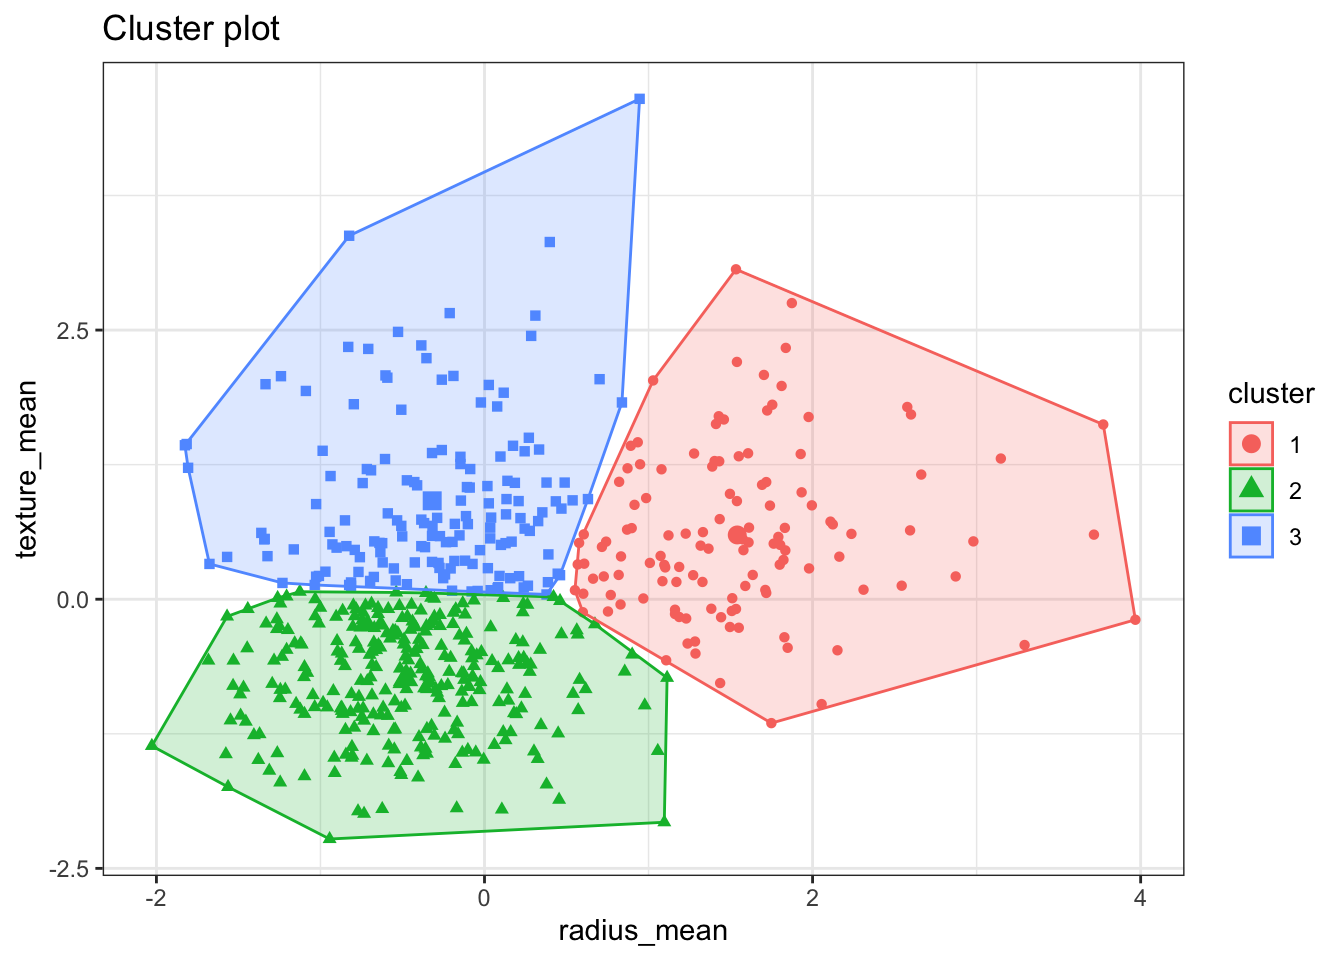
\includegraphics[keepaspectratio]{_main_files/figure-latex/unnamed-chunk-20-1.pdf}}

\textbf{TRY IT YOURSELF:}

\begin{enumerate}
\def\labelenumi{\arabic{enumi})}
\tightlist
\item
  Get 2 clusters with k-mean clustering based on the variables \emph{age},
  \emph{weight}, \emph{height}, \emph{adipos}, \emph{free}, \emph{neck}, \emph{chest},
  \emph{abdom}, \emph{hip}, \emph{thigh}, \emph{knee}, \emph{ankle}, \emph{biceps}, \emph{forearm} and \emph{wrist} .
\end{enumerate}

See the solution code

\begin{Shaded}
\begin{Highlighting}[]
\CommentTok{\#select a subset of the variables}
\NormalTok{bdiag}\FloatTok{.10}\NormalTok{vars }\OtherTok{\textless{}{-}}\NormalTok{ bdiag.data[,}\FunctionTok{c}\NormalTok{(}\StringTok{"radius\_mean"}\NormalTok{, }\StringTok{"texture\_mean"}\NormalTok{,  }
                     \StringTok{"perimeter\_mean"}\NormalTok{, }\StringTok{"area\_mean"}\NormalTok{, }
                     \StringTok{"smoothness\_mean"}\NormalTok{, }\StringTok{"compactness\_mean"}\NormalTok{, }
                     \StringTok{"concavity\_mean"}\NormalTok{, }\StringTok{"concave.points\_mean"}\NormalTok{, }
                     \StringTok{"symmetry\_mean"}\NormalTok{, }\StringTok{"fractal\_dimension\_mean"}\NormalTok{)]}
\NormalTok{k2 }\OtherTok{\textless{}{-}} \FunctionTok{kmeans}\NormalTok{(bdiag}\FloatTok{.10}\NormalTok{vars, }\AttributeTok{centers =} \DecValTok{2}\NormalTok{)}
\FunctionTok{fviz\_cluster}\NormalTok{(k2, }\AttributeTok{data =}\NormalTok{ bdiag}\FloatTok{.10}\NormalTok{vars, }\AttributeTok{label=}\ConstantTok{NA}\NormalTok{)}\SpecialCharTok{+}\FunctionTok{theme\_bw}\NormalTok{()}
\end{Highlighting}
\end{Shaded}

\pandocbounded{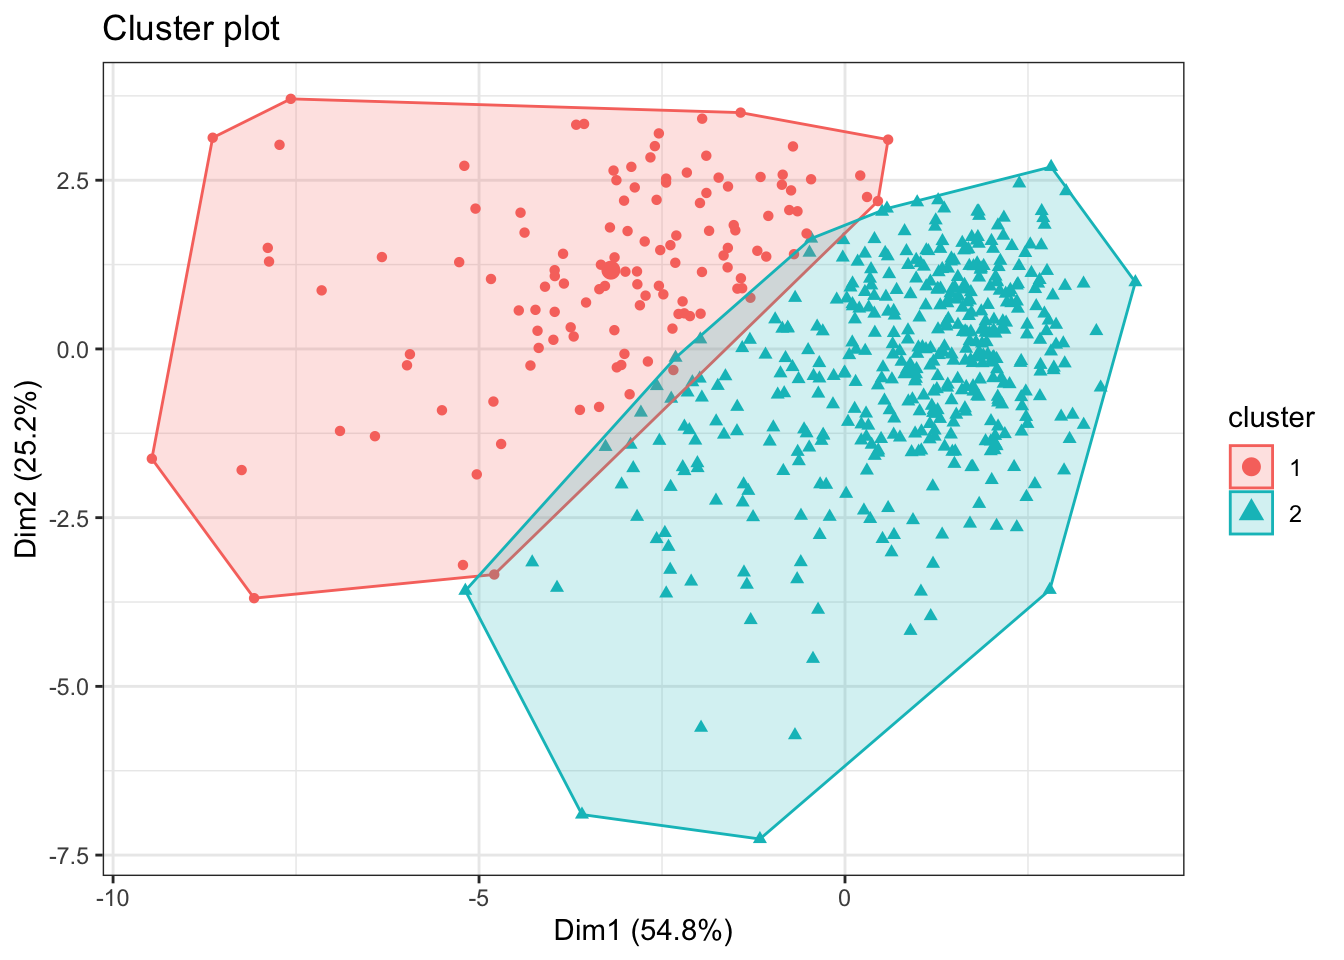
\includegraphics[keepaspectratio]{_main_files/figure-latex/unnamed-chunk-21-1.pdf}}

\subsection*{Task 2 - Choosing the number of clusters}\label{task-2---choosing-the-number-of-clusters}
\addcontentsline{toc}{subsection}{Task 2 - Choosing the number of clusters}

Lets consider the same example as in Task 1 with two variables.How many
clusters should we consider?

There are some ad-hoc visual methods that may help you guide selecting the
number of clusters.

The first method is called the \emph{Elbow method} and consists in

\begin{itemize}
\tightlist
\item
  computing the k-means clustering for different values of \(k\), e.g,
  by varying \(k\) from 1 to 10 clusters
\item
  then, for each k, calculate the total within-cluster sum of square (\(wss\))
\item
  and finally, plot the curve of \(wss\) according to the number of clusters \(k\).
\end{itemize}

In the plot, the location of a bend (knee) suggests the appropriate number
of clusters. The function \texttt{fviz\_nbclust()} implements this method

\begin{Shaded}
\begin{Highlighting}[]
\FunctionTok{fviz\_nbclust}\NormalTok{(bdiag}\FloatTok{.2}\NormalTok{vars, kmeans, }\AttributeTok{method =} \StringTok{"wss"}\NormalTok{,  }\AttributeTok{k.max =} \DecValTok{10}\NormalTok{)}
\end{Highlighting}
\end{Shaded}

\pandocbounded{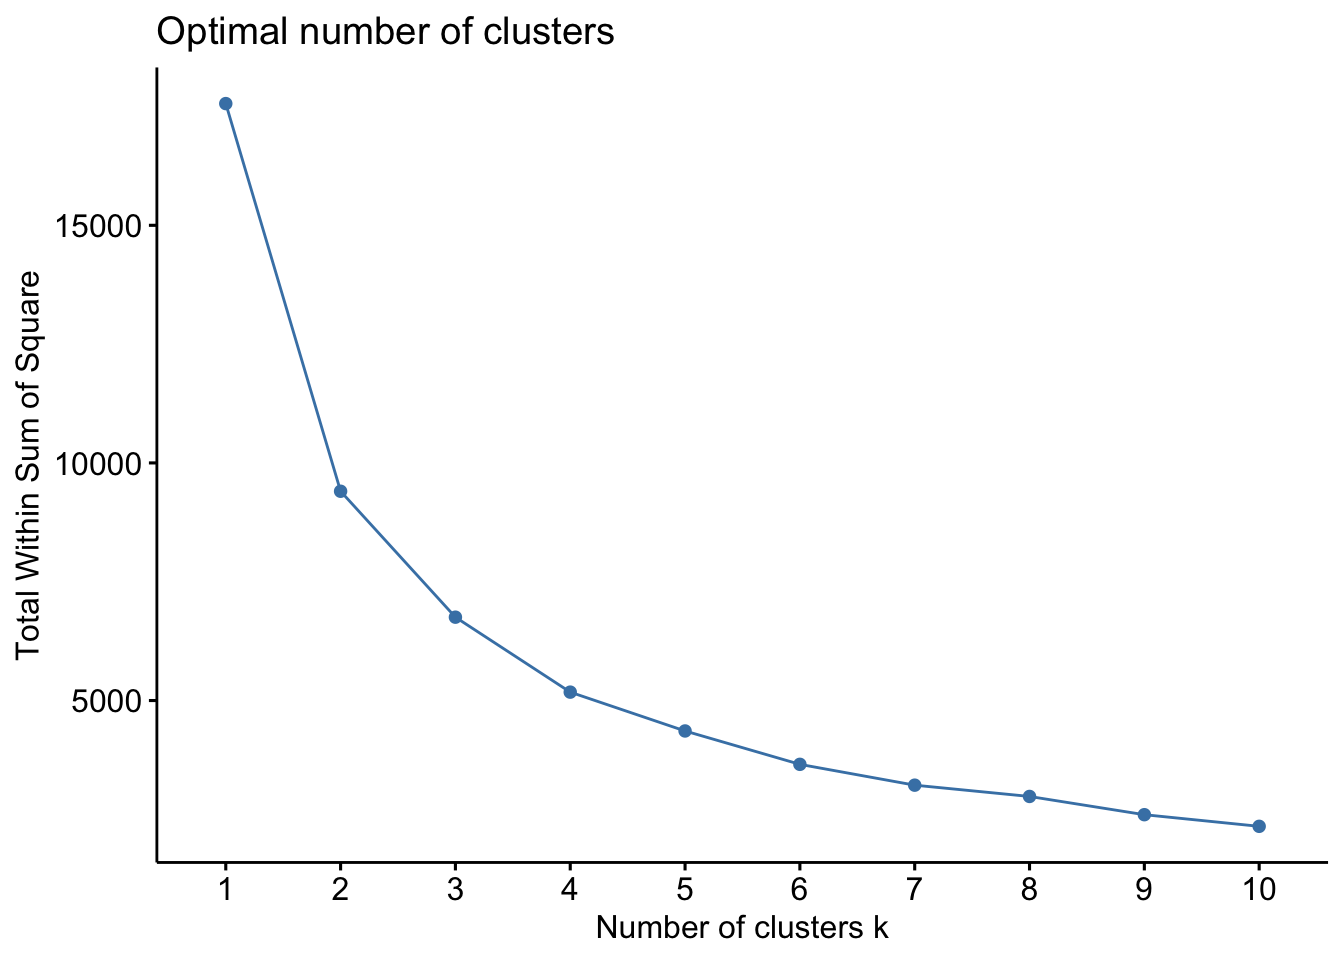
\includegraphics[keepaspectratio]{_main_files/figure-latex/unnamed-chunk-22-1.pdf}}

The plot above suggest 2 or 3 clusters.

Another method is the \textbf{Average Silhouette Method}. In this method we look
at the quality of the clustering by measuring how well each data point lies
within its cluster. If the average silhouette width is high, this suggests
a good clustering.
We can then compute the average silhouette width for different values of \(k\)
and select the number of clusters with higher average silhouette width.

The same function as above also implements this method.

\begin{Shaded}
\begin{Highlighting}[]
\FunctionTok{fviz\_nbclust}\NormalTok{(bdiag}\FloatTok{.2}\NormalTok{vars, kmeans, }\AttributeTok{method =} \StringTok{"silhouette"}\NormalTok{,  }\AttributeTok{k.max =} \DecValTok{10}\NormalTok{)}
\end{Highlighting}
\end{Shaded}

\pandocbounded{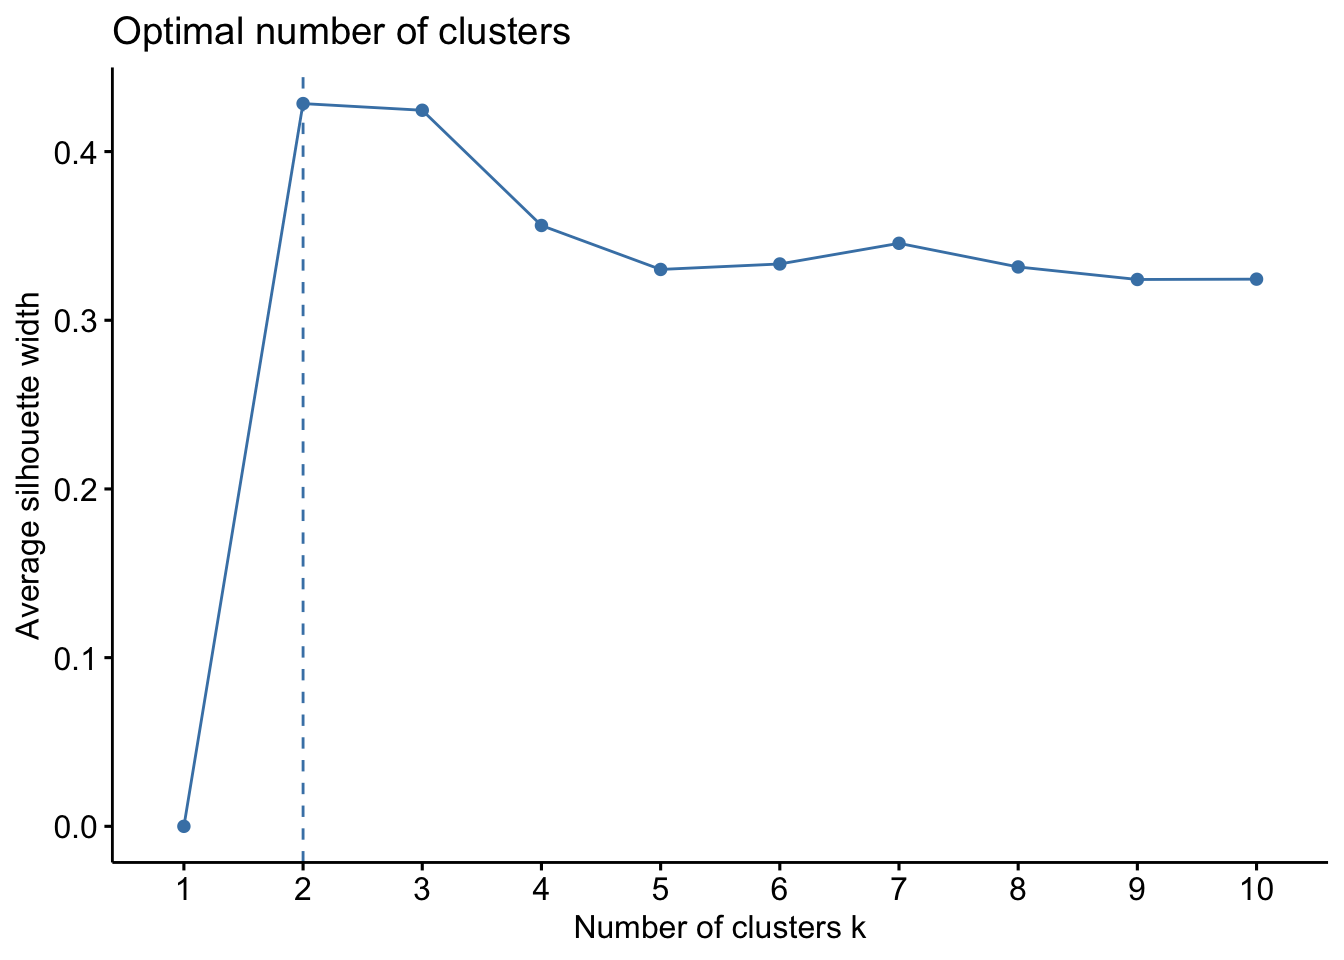
\includegraphics[keepaspectratio]{_main_files/figure-latex/unnamed-chunk-23-1.pdf}}

This method suggests 2 clusters.

The final method is the \textbf{Gap Statistic Method}. This method compares
the total intracluster variation for different number of cluster \(k\)
with their expected values under a data with no clustering (these
data generated using Monte Carlo simulations). The higher the gap between
the observed and expected, the better the clustering.
More details about this method
is available in
\href{http://web.stanford.edu/~hastie/Papers/gap.pdf}{R. Tibshirani, G. Walther, and T. Hastie (Standford University, 2001)}

\begin{Shaded}
\begin{Highlighting}[]
\FunctionTok{fviz\_nbclust}\NormalTok{(bdiag}\FloatTok{.2}\NormalTok{vars, kmeans, }\AttributeTok{method =} \StringTok{"gap"}\NormalTok{,  }\AttributeTok{nboot=}\DecValTok{200}\NormalTok{, }\AttributeTok{k.max =} \DecValTok{10}\NormalTok{)}
\end{Highlighting}
\end{Shaded}

\pandocbounded{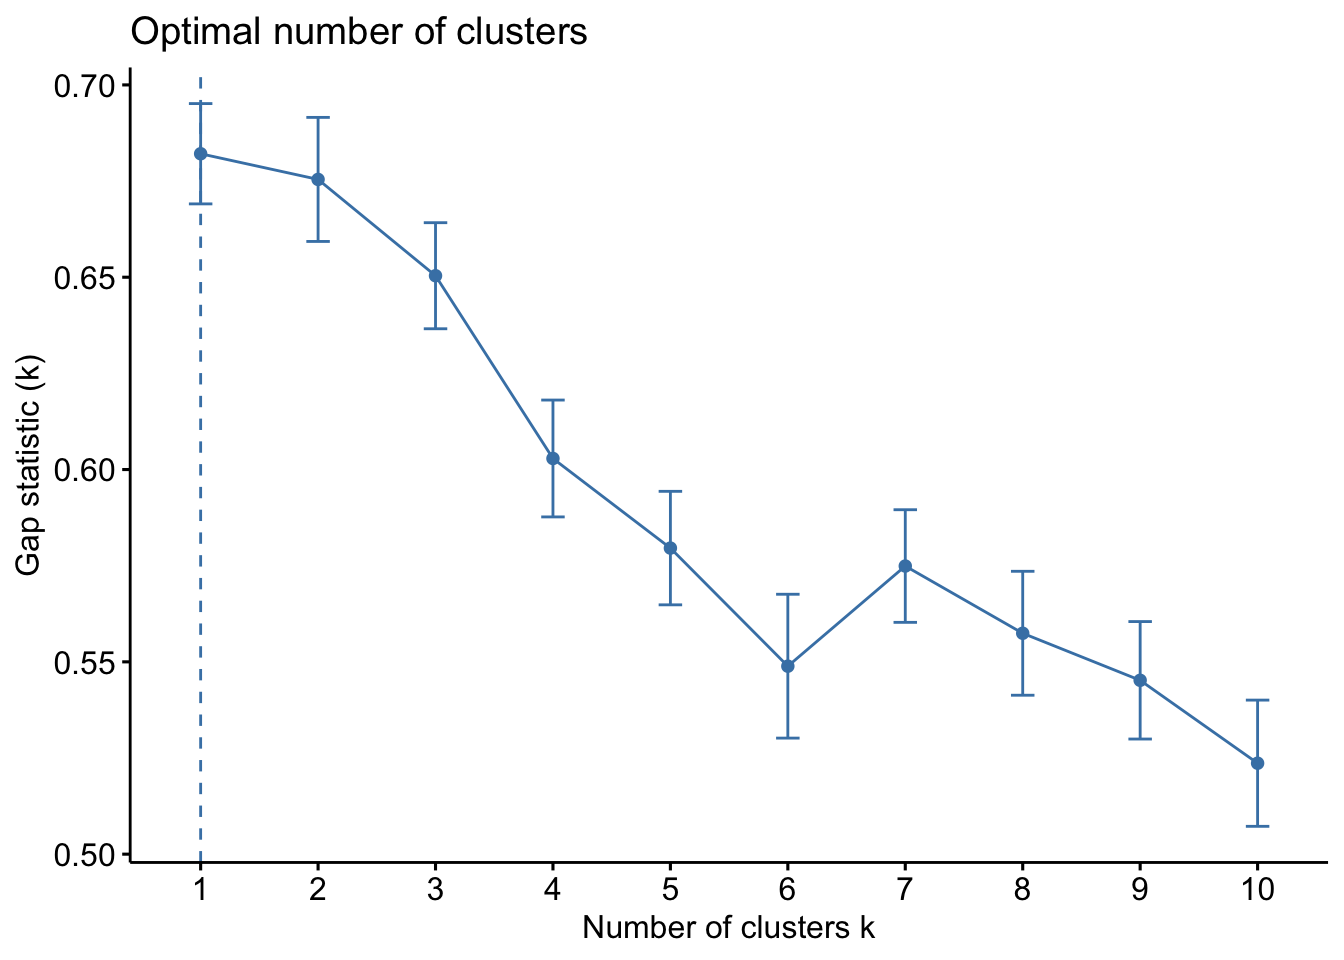
\includegraphics[keepaspectratio]{_main_files/figure-latex/unnamed-chunk-24-1.pdf}}

In this case, the method suggests 1 single cluster.

Depending on the method used, we could have selected between 1 to 3 clusters.

\section{Exercises}\label{KM4}

Solve the following exercises:

\begin{enumerate}
\def\labelenumi{\arabic{enumi})}
\tightlist
\item
  The dataset \emph{fat} is available in the \emph{library(faraway)}.\\
  The dataset contains several physical measurements.
\end{enumerate}

Using the variables \emph{age}, \emph{weight}, \emph{height}, \emph{adipos}, \emph{free}, \emph{neck}, \emph{chest},
\emph{abdom}, \emph{hip}, \emph{thigh}, \emph{knee}, \emph{ankle}, \emph{biceps}, \emph{forearm} and \emph{wrist}

\begin{enumerate}
\def\labelenumi{\alph{enumi})}
\item
  Plot 3 clusters produce by k-mean in the scatter plot formed by the two
  principal components of the data?
\item
  Use different methods to investigate how many clusters are suggested by the
  data.
\end{enumerate}

\chapter{Hierarchical Clustering}\label{hierarchical-clustering}

\section{Introduction}\label{HC1}

\textbf{Hierarchical clustering} is an alternative approach to k-means clustering,which does not require a pre-specification of the number of clusters.

The idea of hierarchical clustering is to treat every observation as its own cluster. Then, at each step, we merge the two clusters that are more similar until all observations are clustered together. This can be represented in a tree shaped image called a \emph{dendrogram}.

\pandocbounded{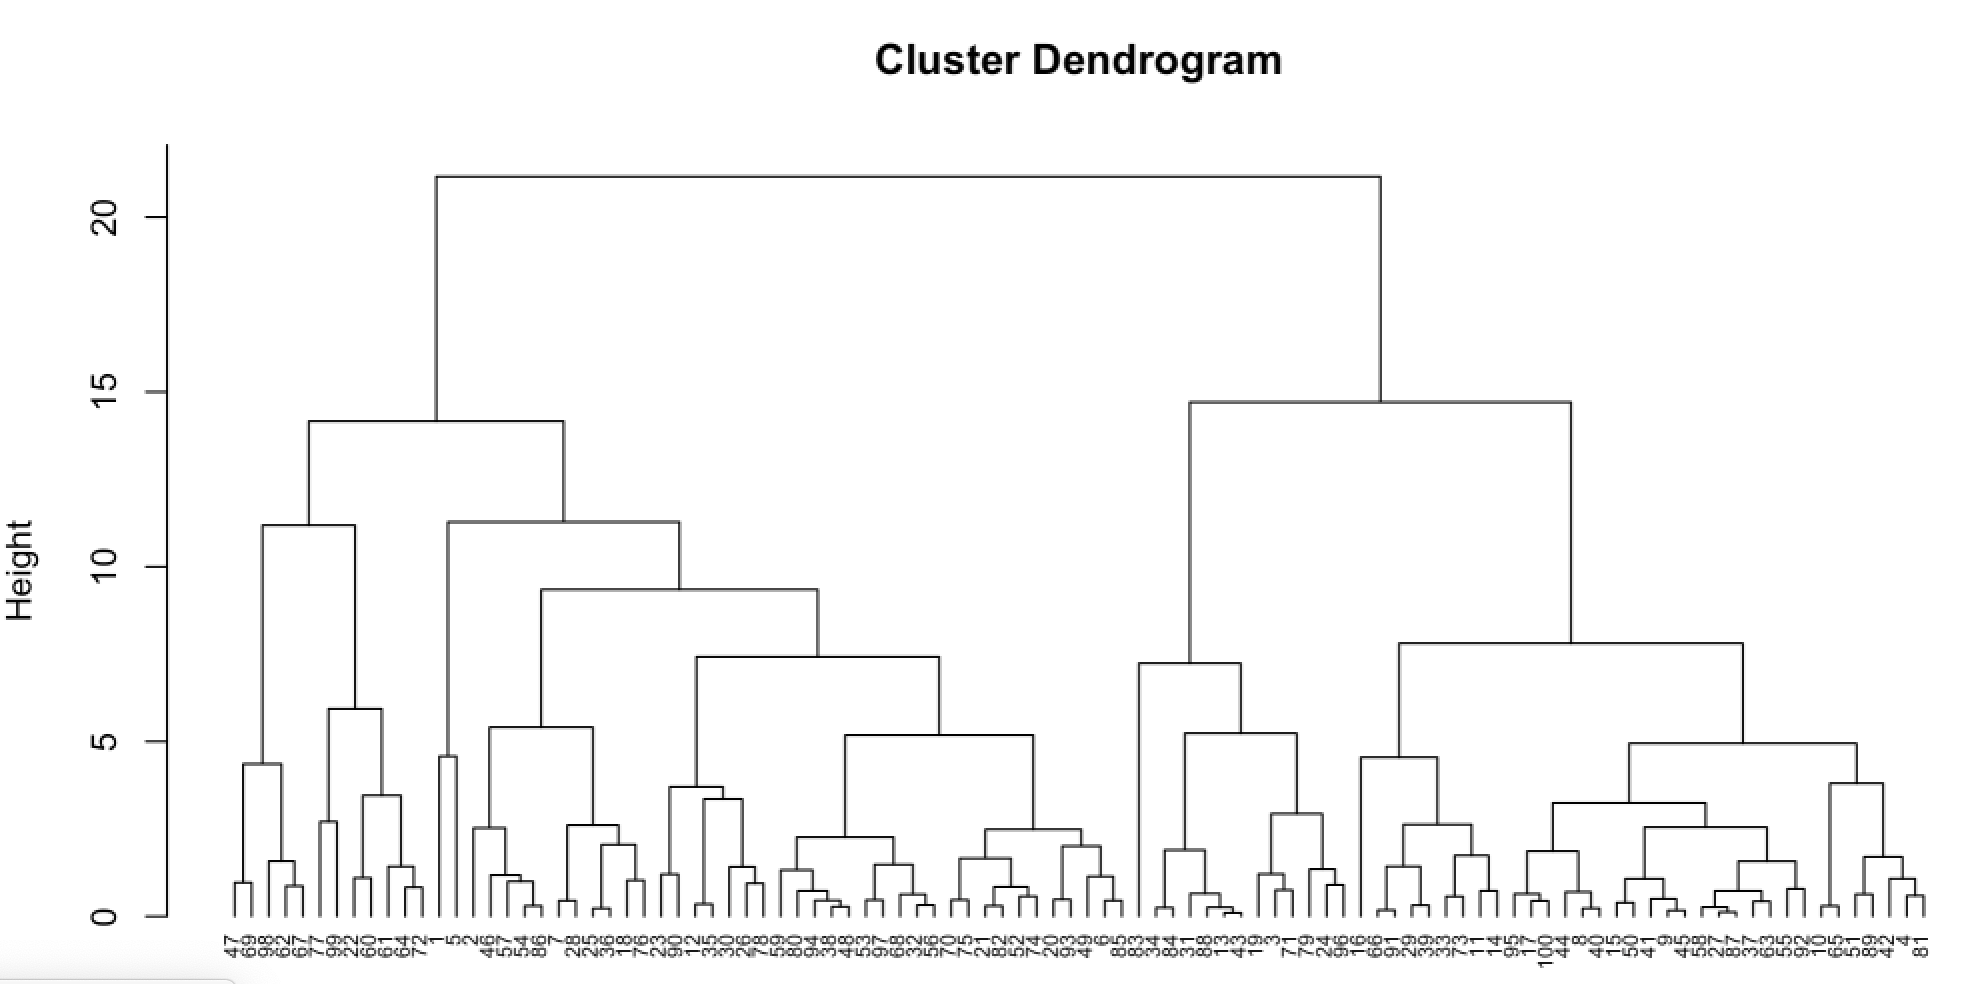
\includegraphics[keepaspectratio]{dendo.png}}

The height of the branches indicate how different the clusters are. The
distance between the groups is usually referred to as \textbf{linkage}. There are
4 types of linkage:

\begin{itemize}
\item
  Complete linkage: It computes all pairwise dissimilarities between the data
  points in cluster A and cluster B. The maximum value of these dissimilarities
  is the distance between the two clusters.
\item
  Single linkage: Similar to complete linkage but it takes the smallest
  (minimum)
  dissimilarity as distance between the two clusters.
\item
  Average linkage: It computes all pairwise dissimilarities between the data
  points in cluster A and cluster B and considers the average of
  these dissimilarities as the distance between the two clusters.
\item
  Centroid linkage clustering: It computes the dissimilarity between the
  centroid for cluster A (a mean vector of length p variables) and the
  centroid for cluster B.
\end{itemize}

Complete and average linkage are more commonly used methods. In terms of
dissimilarity measure, we will use the Euclidean distance but there
are other options.

\section{Readings}\label{HC2}

Read the following chapters of \emph{An introduction to statistical learning}:

\begin{itemize}
\item
  12.4.2 Hierarchical Clustering
\item
  12.4.3 Practical Issues in Clustering
\end{itemize}

\section{Practice session}\label{HC3}

\subsection*{Task 1 - Identify clusters}\label{task-1---identify-clusters}
\addcontentsline{toc}{subsection}{Task 1 - Identify clusters}

Using the \href{https://www.dropbox.com/s/vp44yozebx5xgok/bdiag.csv?dl=1}{bdiag.csv},
let's use 2 of the variables that characterise the cell nuclei: \emph{radius\_mean}
and \emph{texture\_mean} and build a dendrogram

We will use the function \texttt{hclust()} to build the dendrogram and the
function \texttt{dist} that computes the distances between observations:

\begin{Shaded}
\begin{Highlighting}[]
\CommentTok{\#read the dataset}
\NormalTok{bdiag.data }\OtherTok{\textless{}{-}} \FunctionTok{read.csv}\NormalTok{(}\StringTok{"https://www.dropbox.com/s/vp44yozebx5xgok/bdiag.csv?dl=1"}\NormalTok{, }
           \AttributeTok{stringsAsFactors =} \ConstantTok{TRUE}\NormalTok{)}

\CommentTok{\#select a subset of the variables}
\NormalTok{bdiag}\FloatTok{.2}\NormalTok{vars }\OtherTok{\textless{}{-}}\NormalTok{ bdiag.data[,}\FunctionTok{c}\NormalTok{(}\StringTok{"radius\_mean"}\NormalTok{, }\StringTok{"texture\_mean"}\NormalTok{)]}


\CommentTok{\#distances between the observations}
\NormalTok{bdiag.dist }\OtherTok{\textless{}{-}} \FunctionTok{dist}\NormalTok{(bdiag}\FloatTok{.2}\NormalTok{vars, }\AttributeTok{method =} \StringTok{"euclidean"}\NormalTok{)}
      
      \DocumentationTok{\#\#\#\# what is dist() doing?\#\#\#\#\#\#\#\#\#\#\#\#\#\#\#\#\#\#\#\#\#\#\#\#\#\#\#\#\#\#\#\#\#\#}
\NormalTok{      bdiag.dist[}\DecValTok{1}\NormalTok{]  }\CommentTok{\#is the distance between obs1 and obs2}
\end{Highlighting}
\end{Shaded}

\begin{verbatim}
## [1] 7.82742
\end{verbatim}

\begin{Shaded}
\begin{Highlighting}[]
\NormalTok{      bdiag}\FloatTok{.2}\NormalTok{vars[}\DecValTok{1}\SpecialCharTok{:}\DecValTok{2}\NormalTok{, ] }\CommentTok{\#obs 1 and 2}
\end{Highlighting}
\end{Shaded}

\begin{verbatim}
##   radius_mean texture_mean
## 1       17.99        10.38
## 2       20.57        17.77
\end{verbatim}

\begin{Shaded}
\begin{Highlighting}[]
      \FunctionTok{sqrt}\NormalTok{((bdiag}\FloatTok{.2}\NormalTok{vars[}\DecValTok{1}\NormalTok{, }\DecValTok{1}\NormalTok{] }\SpecialCharTok{{-}}\NormalTok{ bdiag}\FloatTok{.2}\NormalTok{vars[}\DecValTok{2}\NormalTok{,}\DecValTok{1}\NormalTok{ ])}\SpecialCharTok{\^{}}\DecValTok{2} \SpecialCharTok{+} 
\NormalTok{        (bdiag}\FloatTok{.2}\NormalTok{vars[}\DecValTok{1}\NormalTok{, }\DecValTok{2}\NormalTok{] }\SpecialCharTok{{-}}\NormalTok{ bdiag}\FloatTok{.2}\NormalTok{vars[}\DecValTok{2}\NormalTok{,}\DecValTok{2}\NormalTok{ ])}\SpecialCharTok{\^{}}\DecValTok{2}\NormalTok{ )  }\CommentTok{\#Eucl distance}
\end{Highlighting}
\end{Shaded}

\begin{verbatim}
## [1] 7.82742
\end{verbatim}

\begin{Shaded}
\begin{Highlighting}[]
      \DocumentationTok{\#\#\#\#\#\#\#\#\#\#\#\#\#\#\#\#\#\#\#\#\#\#\#\#\#\#\#\#\#\#\#\#\#\#\#\#\#\#\#\#\#\#\#\#\#\#\#\#\#\#\#\#\#\#\#\#\#\#\#\#\#}

\CommentTok{\#Dendrogram using the complete linkage method}
\NormalTok{bdiag.ddgram }\OtherTok{\textless{}{-}} \FunctionTok{hclust}\NormalTok{(bdiag.dist, }\AttributeTok{method=}\StringTok{"complete"}\NormalTok{)}
\CommentTok{\#Plot the dendrogram}
\CommentTok{\#the option hang = {-}1 will make the}
\CommentTok{\#labels appear below 0}
\FunctionTok{plot}\NormalTok{(bdiag.ddgram, }\AttributeTok{cex=}\NormalTok{.}\DecValTok{4}\NormalTok{, }\AttributeTok{hang =} \SpecialCharTok{{-}}\DecValTok{1}\NormalTok{)}
\end{Highlighting}
\end{Shaded}

\pandocbounded{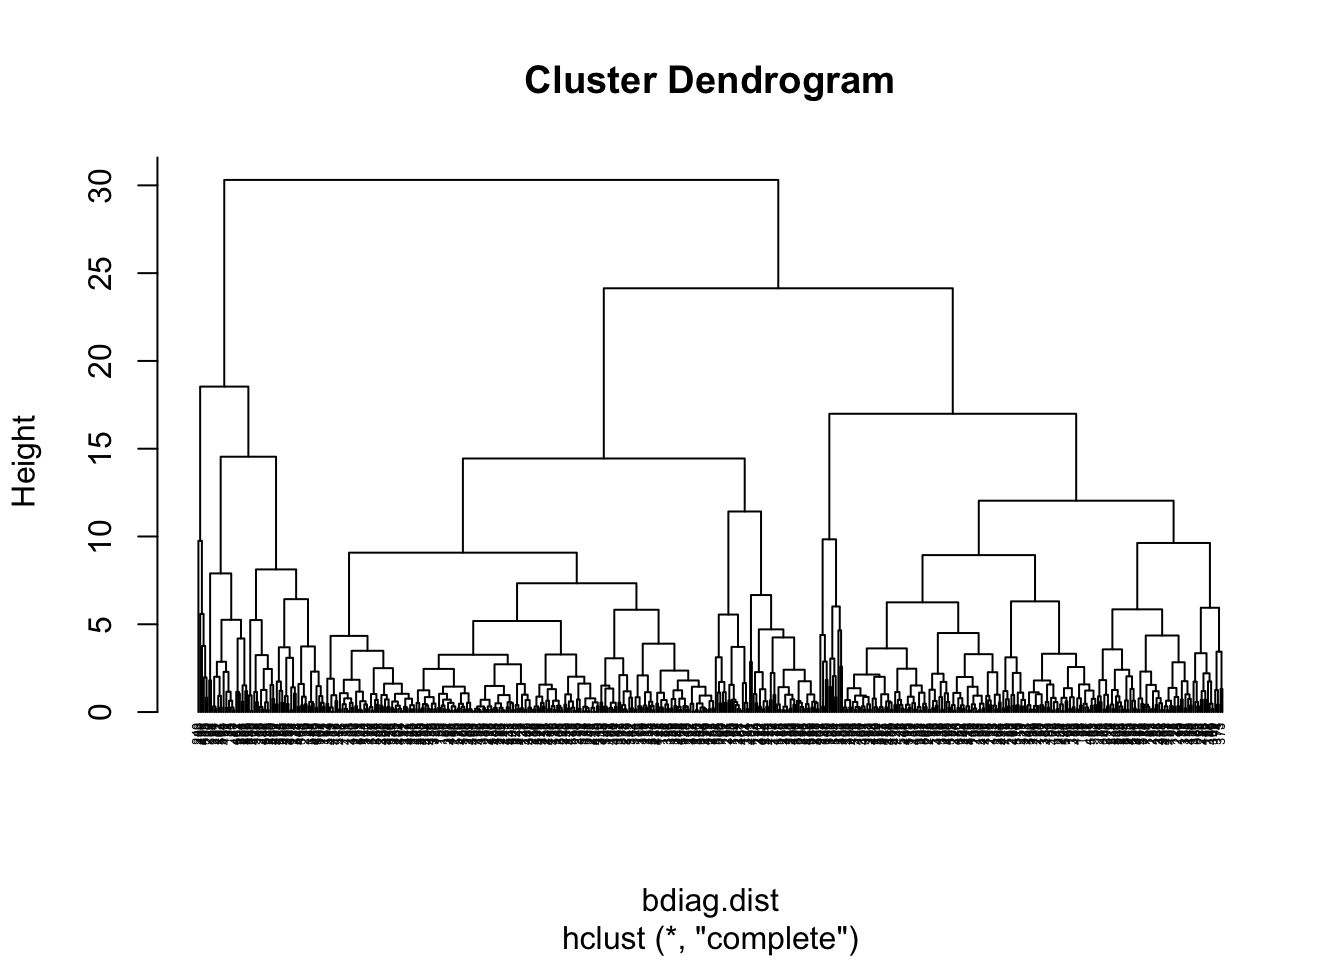
\includegraphics[keepaspectratio]{_main_files/figure-latex/unnamed-chunk-26-1.pdf}}

If we cut the tree at the height of 20, we get 3 clusters

\begin{Shaded}
\begin{Highlighting}[]
\FunctionTok{plot}\NormalTok{(bdiag.ddgram, }\AttributeTok{cex=}\NormalTok{.}\DecValTok{4}\NormalTok{, }\AttributeTok{hang =} \SpecialCharTok{{-}}\DecValTok{1}\NormalTok{)}
\FunctionTok{abline}\NormalTok{(}\AttributeTok{a=}\DecValTok{20}\NormalTok{, }\AttributeTok{b=}\DecValTok{0}\NormalTok{, }\AttributeTok{lty=}\DecValTok{2}\NormalTok{)}
\end{Highlighting}
\end{Shaded}

\pandocbounded{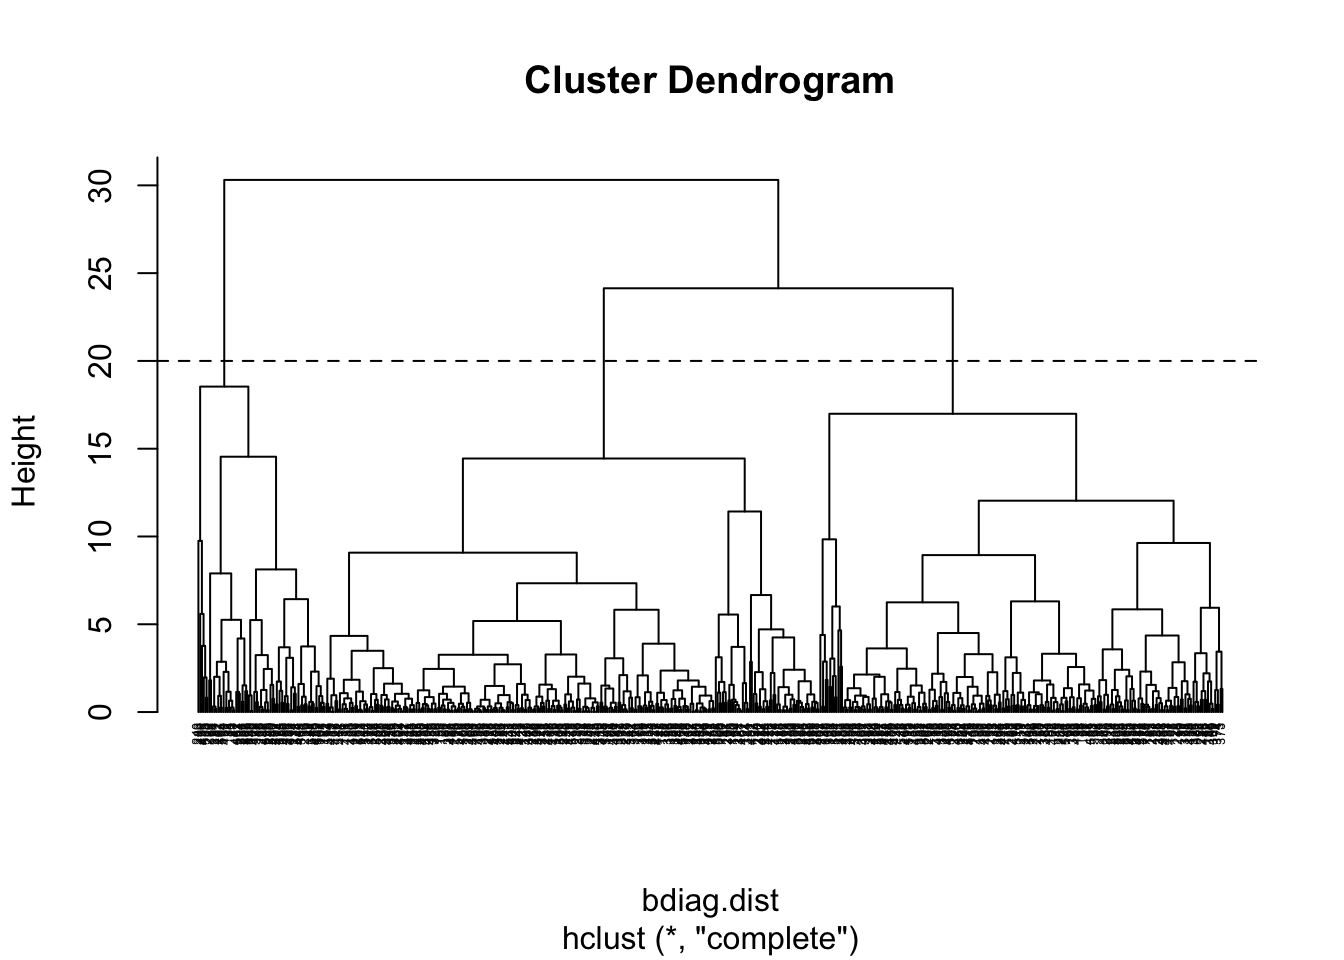
\includegraphics[keepaspectratio]{_main_files/figure-latex/unnamed-chunk-27-1.pdf}}

We can draw a rectangle around the 3 clusters

\begin{Shaded}
\begin{Highlighting}[]
\FunctionTok{plot}\NormalTok{(bdiag.ddgram, }\AttributeTok{cex=}\NormalTok{.}\DecValTok{4}\NormalTok{, }\AttributeTok{hang =} \SpecialCharTok{{-}}\DecValTok{1}\NormalTok{)}
\FunctionTok{rect.hclust}\NormalTok{(bdiag.ddgram, }\AttributeTok{k =} \DecValTok{3}\NormalTok{, }\AttributeTok{border =} \DecValTok{2}\SpecialCharTok{:}\DecValTok{5}\NormalTok{)}
\end{Highlighting}
\end{Shaded}

\pandocbounded{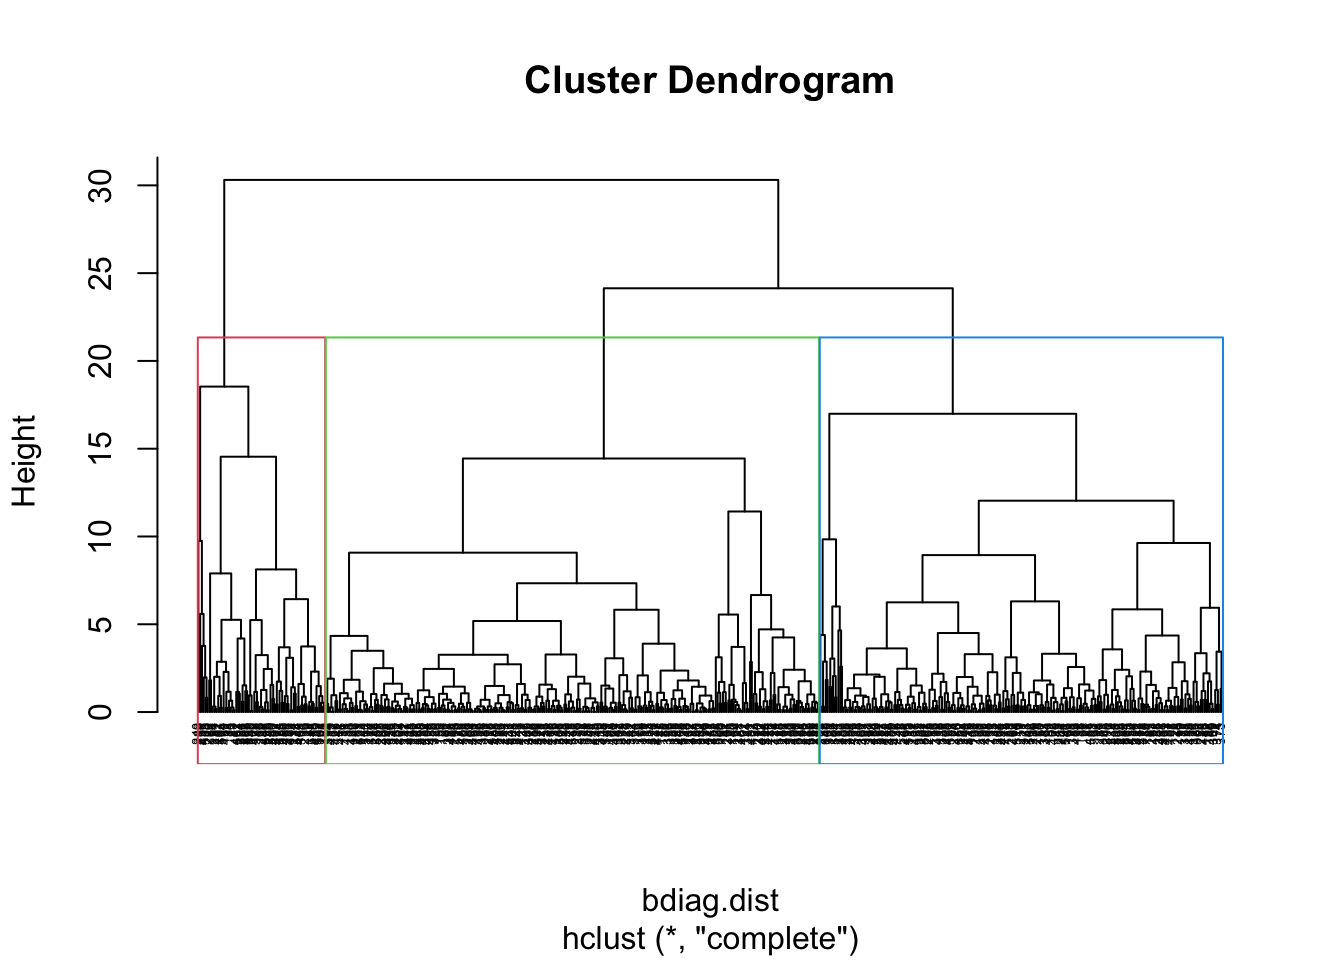
\includegraphics[keepaspectratio]{_main_files/figure-latex/unnamed-chunk-28-1.pdf}}

And obtain the cluster for each observation

\begin{Shaded}
\begin{Highlighting}[]
\NormalTok{group3 }\OtherTok{\textless{}{-}} \FunctionTok{cutree}\NormalTok{(bdiag.ddgram, }\AttributeTok{k =} \DecValTok{2}\NormalTok{)  }
\FunctionTok{table}\NormalTok{(group3 )}
\end{Highlighting}
\end{Shaded}

\begin{verbatim}
## group3
##   1   2 
## 498  71
\end{verbatim}

\begin{Shaded}
\begin{Highlighting}[]
\CommentTok{\#We can also visualise the clusters}
\FunctionTok{fviz\_cluster}\NormalTok{(}\FunctionTok{list}\NormalTok{(}\AttributeTok{data =}\NormalTok{ bdiag}\FloatTok{.2}\NormalTok{vars, }\AttributeTok{cluster =}\NormalTok{ group3 ))}
\end{Highlighting}
\end{Shaded}

\pandocbounded{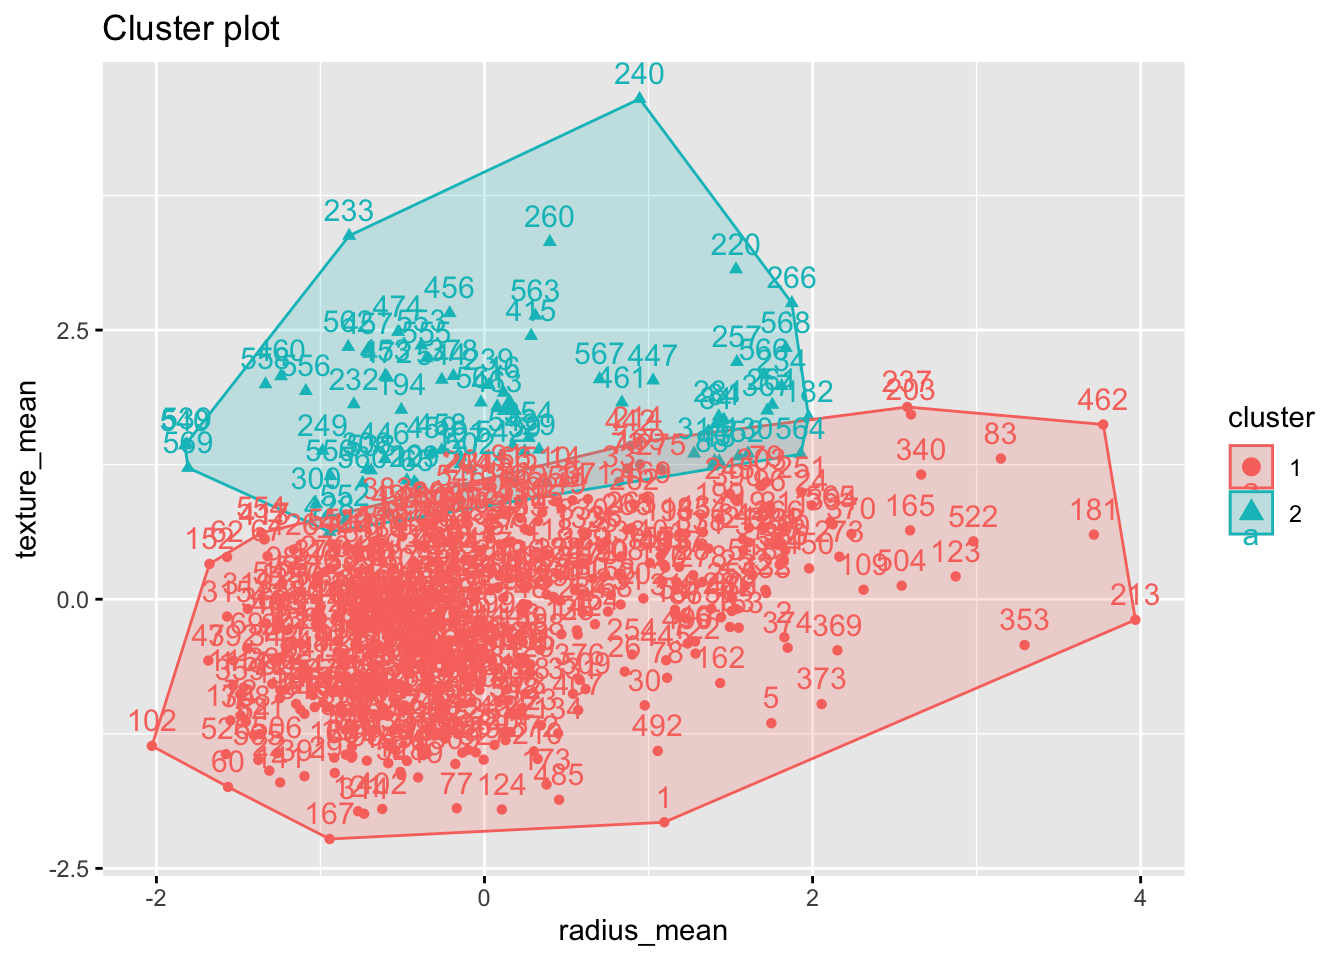
\includegraphics[keepaspectratio]{_main_files/figure-latex/unnamed-chunk-29-1.pdf}}

\textbf{TRY IT YOURSELF:}

\begin{enumerate}
\def\labelenumi{\arabic{enumi})}
\tightlist
\item
  Get 2 clusters with hierachical clustering using the variables \emph{age},
  \emph{weight}, \emph{height}, \emph{adipos}, \emph{free}, \emph{neck}, \emph{chest},
  \emph{abdom}, \emph{hip}, \emph{thigh}, \emph{knee}, \emph{ankle}, \emph{biceps}, \emph{forearm} and \emph{wrist}.
  and compare the clustering result with the observed \emph{diagnosis}
\end{enumerate}

See the solution code

\begin{Shaded}
\begin{Highlighting}[]
\CommentTok{\#select a subset of the variables}
\NormalTok{bdiag}\FloatTok{.10}\NormalTok{vars }\OtherTok{\textless{}{-}}\NormalTok{ bdiag.data[,}\FunctionTok{c}\NormalTok{(}\StringTok{"radius\_mean"}\NormalTok{, }\StringTok{"texture\_mean"}\NormalTok{,  }
                     \StringTok{"perimeter\_mean"}\NormalTok{, }\StringTok{"area\_mean"}\NormalTok{, }
                     \StringTok{"smoothness\_mean"}\NormalTok{, }\StringTok{"compactness\_mean"}\NormalTok{, }
                     \StringTok{"concavity\_mean"}\NormalTok{, }\StringTok{"concave.points\_mean"}\NormalTok{, }
                     \StringTok{"symmetry\_mean"}\NormalTok{, }\StringTok{"fractal\_dimension\_mean"}\NormalTok{)]}

\CommentTok{\#distances between the observations}
\NormalTok{bdiag.dist10 }\OtherTok{\textless{}{-}} \FunctionTok{dist}\NormalTok{(bdiag}\FloatTok{.10}\NormalTok{vars, }\AttributeTok{method =} \StringTok{"euclidean"}\NormalTok{)}
\CommentTok{\#Dendrogram using the complete linkage method}
\NormalTok{bdiag.ddgram10 }\OtherTok{\textless{}{-}} \FunctionTok{hclust}\NormalTok{(bdiag.dist10, }\AttributeTok{method=}\StringTok{"complete"}\NormalTok{)}
\FunctionTok{plot}\NormalTok{(bdiag.ddgram, }\AttributeTok{cex=}\NormalTok{.}\DecValTok{4}\NormalTok{, }\AttributeTok{hang =} \SpecialCharTok{{-}}\DecValTok{1}\NormalTok{)}
\end{Highlighting}
\end{Shaded}

\pandocbounded{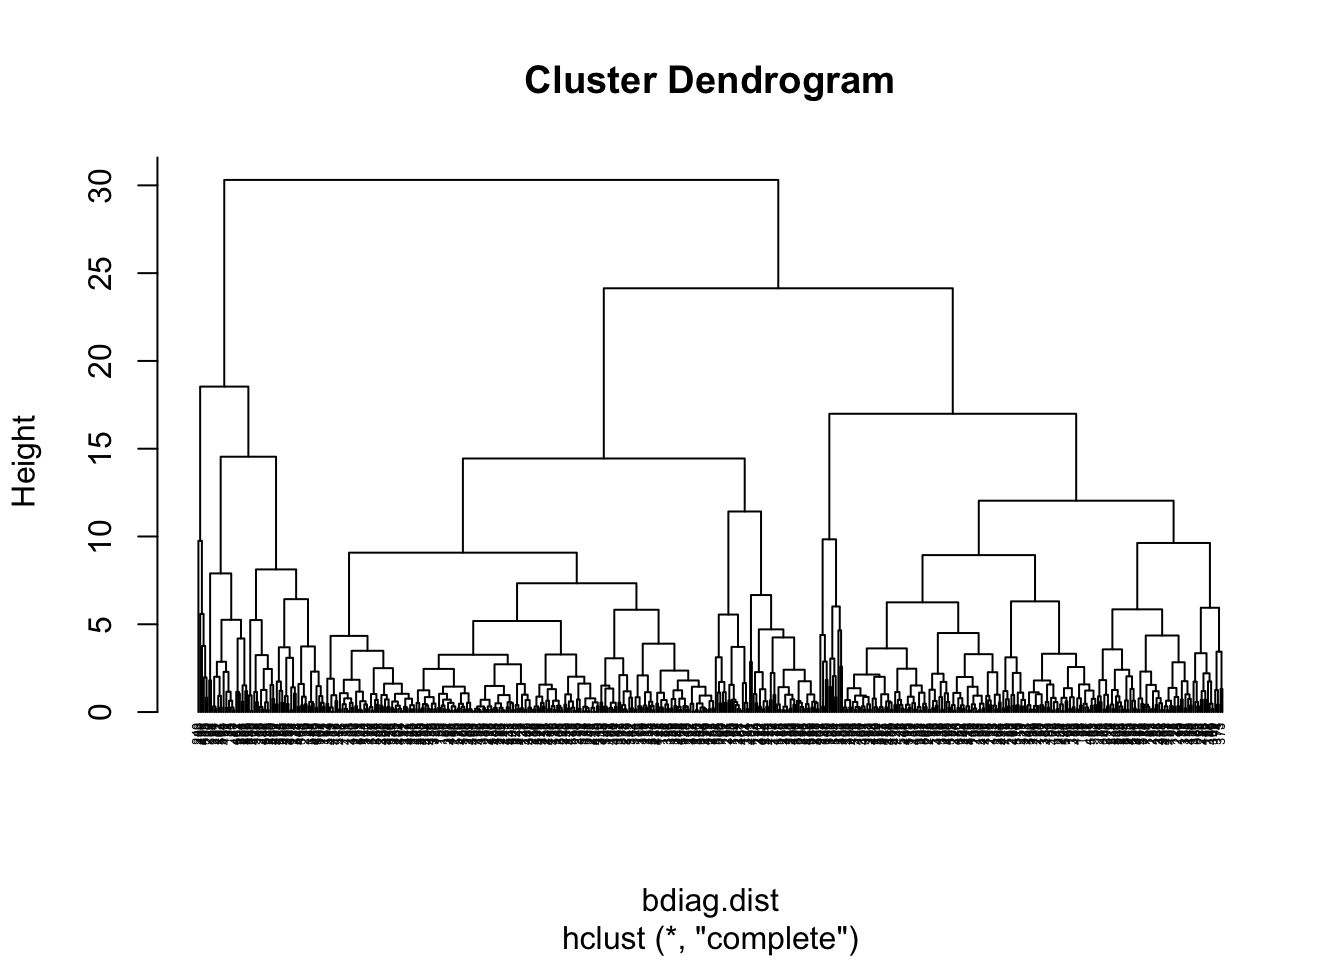
\includegraphics[keepaspectratio]{_main_files/figure-latex/unnamed-chunk-30-1.pdf}}

\begin{Shaded}
\begin{Highlighting}[]
\NormalTok{bdiag}\FloatTok{.2}\NormalTok{vars}\SpecialCharTok{$}\NormalTok{cluster }\OtherTok{\textless{}{-}} \FunctionTok{cutree}\NormalTok{(bdiag.ddgram10, }\AttributeTok{k =} \DecValTok{2}\NormalTok{)  }
\FunctionTok{table}\NormalTok{(bdiag}\FloatTok{.2}\NormalTok{vars}\SpecialCharTok{$}\NormalTok{cluster, bdiag.data}\SpecialCharTok{$}\NormalTok{diagnosis)}
\end{Highlighting}
\end{Shaded}

\begin{enumerate}
\def\labelenumi{\arabic{enumi})}
\setcounter{enumi}{1}
\tightlist
\item
  How does the clustering changes with different linkage methods?
\end{enumerate}

See the solution code

\begin{Shaded}
\begin{Highlighting}[]
\CommentTok{\#select a subset of the variables}
\NormalTok{bdiag}\FloatTok{.10}\NormalTok{vars }\OtherTok{\textless{}{-}}\NormalTok{ bdiag.data[,}\FunctionTok{c}\NormalTok{(}\StringTok{"radius\_mean"}\NormalTok{, }\StringTok{"texture\_mean"}\NormalTok{,  }
                     \StringTok{"perimeter\_mean"}\NormalTok{, }\StringTok{"area\_mean"}\NormalTok{, }
                     \StringTok{"smoothness\_mean"}\NormalTok{, }\StringTok{"compactness\_mean"}\NormalTok{, }
                     \StringTok{"concavity\_mean"}\NormalTok{, }\StringTok{"concave.points\_mean"}\NormalTok{, }
                     \StringTok{"symmetry\_mean"}\NormalTok{, }\StringTok{"fractal\_dimension\_mean"}\NormalTok{)]}

\CommentTok{\#distances between the observations}
\NormalTok{bdiag.dist10 }\OtherTok{\textless{}{-}} \FunctionTok{dist}\NormalTok{(bdiag}\FloatTok{.10}\NormalTok{vars, }\AttributeTok{method =} \StringTok{"euclidean"}\NormalTok{)}
\CommentTok{\#Dendrogram using the complete linkage method}
\NormalTok{bdiag.ddgram10.comp }\OtherTok{\textless{}{-}} \FunctionTok{hclust}\NormalTok{(bdiag.dist10, }\AttributeTok{method=}\StringTok{"complete"}\NormalTok{)}
\NormalTok{bdiag.ddgram10.sing }\OtherTok{\textless{}{-}} \FunctionTok{hclust}\NormalTok{(bdiag.dist10, }\AttributeTok{method=}\StringTok{"single"}\NormalTok{)}
\NormalTok{bdiag.ddgram10.aver }\OtherTok{\textless{}{-}}  \FunctionTok{hclust}\NormalTok{(bdiag.dist10, }\AttributeTok{method=}\StringTok{"average"}\NormalTok{)}
\NormalTok{bdiag.ddgram10.cent }\OtherTok{\textless{}{-}}  \FunctionTok{hclust}\NormalTok{(bdiag.dist10, }\AttributeTok{method=}\StringTok{"centroid"}\NormalTok{)}

\NormalTok{bdiag}\FloatTok{.2}\NormalTok{vars}\SpecialCharTok{$}\NormalTok{cluster.comp }\OtherTok{\textless{}{-}} \FunctionTok{cutree}\NormalTok{(bdiag.ddgram10.comp, }\AttributeTok{k =} \DecValTok{2}\NormalTok{)  }
\NormalTok{bdiag}\FloatTok{.2}\NormalTok{vars}\SpecialCharTok{$}\NormalTok{cluster.sing }\OtherTok{\textless{}{-}} \FunctionTok{cutree}\NormalTok{(bdiag.ddgram10.sing, }\AttributeTok{k =} \DecValTok{2}\NormalTok{)  }
\NormalTok{bdiag}\FloatTok{.2}\NormalTok{vars}\SpecialCharTok{$}\NormalTok{cluster.aver }\OtherTok{\textless{}{-}} \FunctionTok{cutree}\NormalTok{(bdiag.ddgram10.aver, }\AttributeTok{k =} \DecValTok{2}\NormalTok{)  }
\NormalTok{bdiag}\FloatTok{.2}\NormalTok{vars}\SpecialCharTok{$}\NormalTok{cluster.cent }\OtherTok{\textless{}{-}} \FunctionTok{cutree}\NormalTok{(bdiag.ddgram10.cent, }\AttributeTok{k =} \DecValTok{2}\NormalTok{)  }

\FunctionTok{table}\NormalTok{(bdiag}\FloatTok{.2}\NormalTok{vars}\SpecialCharTok{$}\NormalTok{cluster.comp, bdiag}\FloatTok{.2}\NormalTok{vars}\SpecialCharTok{$}\NormalTok{cluster.sing)}
\FunctionTok{table}\NormalTok{(bdiag}\FloatTok{.2}\NormalTok{vars}\SpecialCharTok{$}\NormalTok{cluster.comp, bdiag}\FloatTok{.2}\NormalTok{vars}\SpecialCharTok{$}\NormalTok{cluster.aver)}
\FunctionTok{table}\NormalTok{(bdiag}\FloatTok{.2}\NormalTok{vars}\SpecialCharTok{$}\NormalTok{cluster.comp, bdiag}\FloatTok{.2}\NormalTok{vars}\SpecialCharTok{$}\NormalTok{cluster.cent)}
\end{Highlighting}
\end{Shaded}

\section{Exercises}\label{HC4}

Solve the following exercises:

\begin{enumerate}
\def\labelenumi{\arabic{enumi})}
\tightlist
\item
  The dataset \emph{fat} is available in the \emph{library(faraway)}.\\
  The dataset contains several physical measurements.
\end{enumerate}

Using the variables \emph{age}, \emph{weight}, \emph{height}, \emph{adipos}, \emph{free}, \emph{neck}, \emph{chest},
\emph{abdom}, \emph{hip}, \emph{thigh}, \emph{knee}, \emph{ankle}, \emph{biceps}, \emph{forearm} and \emph{wrist}

\begin{enumerate}
\def\labelenumi{\alph{enumi})}
\item
  Plot 3 clusters produce by hierarchical cluster based on the two
  principal components of the data?
\item
  Compare the result above with the
  clusters obtained using all the variables.
\end{enumerate}

\end{document}
